\pdfoutput=1
%% Author: PGL  Porta Mana
%% Created: 2018-06-25T13:53:29+0200
%% Last-Updated: 2018-07-21T11:39:27+0200
%%%%%%%%%%%%%%%%%%%%%%%%%%%%%%%%%%%%%%%%%%%%%%%%%%%%%%%%%%%%%%%%%%%%%%
% Report-no: ***
\newif\ifarxiv
\arxivfalse
\ifarxiv\pdfmapfile{+classico.map}\fi
\newif\ifafour
\afourfalse % true = A4, false = A5
\newif\iftypodisclaim % typographical disclaim on the side
\typodisclaimtrue
\newif\ifpublic
\publictrue % true = for publication, false = personal notes
\newcommand*{\memfontfamily}{zplx}
\newcommand*{\memfontpack}{newpxtext}
\documentclass[\ifafour a4paper,12pt,\else a5paper,10pt,\fi%extrafontsizes,%
onecolumn,oneside,article,%french,italian,german,swedish,latin,
british%
]{memoir}
\newcommand*{\updated}{\today}
\newcommand*{\firstdraft}{25 June 2018}
\newcommand*{\firstpublished}{\today}
\newcommand*{\propertitle}{Parameter priors for Ising models\\{\large
    research notes}}
\newcommand*{\pdftitle}{Parameter priors for Ising models}
\newcommand*{\headtitle}{Priors for Ising models}
\newcommand*{\pdfauthor}{P.G.L.  Porta Mana, Y. Roudi}
\newcommand*{\headauthor}{\ifpublic Porta Mana, Roudi%
\else Luca\fi}
\newcommand*{\reporthead}{}%Open Science Framework \osfeprint{***}}
%%%%%%%%%%%%%%%%%%%%%%%%%%%%%%%%%%%%%%%%%%%%%%%%%%%%%%%%%%%%%%%%%%%%%%%%%%%%
%%%%%%%%%%%%%%%%%%%%%%%%%%%%%%%%%%%%%%%%%%%%%%%%%%%%%%%%%%%%%%%%%%%%%%%%%%%%
%\usepackage{pifont}
%\usepackage{fontawesome}
\usepackage[T1]{fontenc} 
\input{glyphtounicode} \pdfgentounicode=1
\usepackage[utf8]{inputenx}
%\usepackage{newunicodechar}
% \newunicodechar{Ĕ}{\u{E}}
% \newunicodechar{ĕ}{\u{e}}
% \newunicodechar{Ĭ}{\u{I}}
% \newunicodechar{ĭ}{\u{\i}}
% \newunicodechar{Ŏ}{\u{O}}
% \newunicodechar{ŏ}{\u{o}}
% \newunicodechar{Ŭ}{\u{U}}
% \newunicodechar{ŭ}{\u{u}}
% \newunicodechar{Ā}{\=A}
% \newunicodechar{ā}{\=a}
% \newunicodechar{Ē}{\=E}
% \newunicodechar{ē}{\=e}
% \newunicodechar{Ī}{\=I}
% \newunicodechar{ī}{\={\i}}
% \newunicodechar{Ō}{\=O}
% \newunicodechar{ō}{\=o}
% \newunicodechar{Ū}{\=U}
% \newunicodechar{ū}{\=u}
% \newunicodechar{Ȳ}{\=Y}
% \newunicodechar{ȳ}{\=y}

\newcommand*{\bmmax}{0} % reduce number of bold fonts, before bm
\newcommand*{\hmmax}{0} % reduce number of heavy fonts, before bm
\usepackage{textcomp}
\usepackage[normalem]{ulem}
% \makeatletter
% \def\ssout{\bgroup \ULdepth=-.35ex%\UL@setULdepth
%  \markoverwith{\lower\ULdepth\hbox
%    {\kern-.03em\vbox{\hrule width.2em\kern1.2\p@\hrule}\kern-.03em}}%
%  \ULon}
% \makeatother
\usepackage{amsmath}
\usepackage{mathtools}
\addtolength{\jot}{\jot} % increase spacing in multiline formulae
\usepackage{empheq}% automatically calls amsmath and mathtools
\newcommand*{\widefbox}[1]{\fbox{\hspace{1em}#1\hspace{1em}}}
\setlength{\multlinegap}{0pt}
%\usepackage{fancybox}
\usepackage{framed}
% \usepackage[misc]{ifsym} % for dice
% \newcommand*{\diceone}{{\scriptsize\Cube{1}}}
\usepackage{amssymb}
\usepackage{amsxtra}

\usepackage[main=british,french,italian,german,swedish,latin,esperanto]{babel}\selectlanguage{british}
\newcommand*{\langfrench}{\foreignlanguage{french}}
\newcommand*{\langgerman}{\foreignlanguage{german}}
\newcommand*{\langitalian}{\foreignlanguage{italian}}
\newcommand*{\langswedish}{\foreignlanguage{swedish}}
\newcommand*{\langlatin}{\foreignlanguage{latin}}
\newcommand*{\langnohyph}{\foreignlanguage{nohyphenation}}

\usepackage[autostyle=false,autopunct=false,english=british]{csquotes}
\setquotestyle{british}

\usepackage{amsthm}
\newcommand*{\QED}{\textsc{q.e.d.}}
\renewcommand*{\qedsymbol}{\QED}
\theoremstyle{remark}
\newtheorem{note}{Note}
\newtheorem*{remark}{Note}
\newtheoremstyle{innote}{\parsep}{\parsep}{\footnotesize}{}{}{}{0pt}{}
\theoremstyle{innote}
\newtheorem*{innote}{}


\usepackage[shortlabels,inline]{enumitem}
\SetEnumitemKey{para}{itemindent=\parindent,leftmargin=0pt,listparindent=\parindent,parsep=0pt,itemsep=\topsep}
% \begin{asparaenum} = \begin{enumerate}[para]
% \begin{inparaenum} = \begin{enumerate*}
\setlist[enumerate,2]{label=\alph*.}
\setlist[enumerate]{label=\arabic*.,leftmargin=1.5\parindent}
\setlist[itemize]{leftmargin=1.5\parindent}
\setlist[description]{leftmargin=1.5\parindent}

\usepackage[babel,theoremfont]{newpxtext}
\usepackage[bigdelims,nosymbolsc%,smallerops % probably arXiv doesn't have it
]{newpxmath}
\useosf\linespread{1.083}
%% smaller operators for old version of newpxmath
\makeatletter
\def\re@DeclareMathSymbol#1#2#3#4{%
    \let#1=\undefined
    \DeclareMathSymbol{#1}{#2}{#3}{#4}}
%\re@DeclareMathSymbol{\bigsqcupop}{\mathop}{largesymbols}{"46}
%\re@DeclareMathSymbol{\bigodotop}{\mathop}{largesymbols}{"4A}
\re@DeclareMathSymbol{\bigoplusop}{\mathop}{largesymbols}{"4C}
\re@DeclareMathSymbol{\bigotimesop}{\mathop}{largesymbols}{"4E}
\re@DeclareMathSymbol{\sumop}{\mathop}{largesymbols}{"50}
\re@DeclareMathSymbol{\prodop}{\mathop}{largesymbols}{"51}
\re@DeclareMathSymbol{\bigcupop}{\mathop}{largesymbols}{"53}
\re@DeclareMathSymbol{\bigcapop}{\mathop}{largesymbols}{"54}
%\re@DeclareMathSymbol{\biguplusop}{\mathop}{largesymbols}{"55}
\re@DeclareMathSymbol{\bigwedgeop}{\mathop}{largesymbols}{"56}
\re@DeclareMathSymbol{\bigveeop}{\mathop}{largesymbols}{"57}
%\re@DeclareMathSymbol{\bigcupdotop}{\mathop}{largesymbols}{"DF}
%\re@DeclareMathSymbol{\bigcapplusop}{\mathop}{largesymbolsPXA}{"00}
%\re@DeclareMathSymbol{\bigsqcupplusop}{\mathop}{largesymbolsPXA}{"02}
%\re@DeclareMathSymbol{\bigsqcapplusop}{\mathop}{largesymbolsPXA}{"04}
%\re@DeclareMathSymbol{\bigsqcapop}{\mathop}{largesymbolsPXA}{"06}
\re@DeclareMathSymbol{\bigtimesop}{\mathop}{largesymbolsPXA}{"10}
%\re@DeclareMathSymbol{\coprodop}{\mathop}{largesymbols}{"60}
%\re@DeclareMathSymbol{\varprod}{\mathop}{largesymbolsPXA}{16}
\makeatother


%% With euler font cursive for Greek letters - the [1] means 100% scaling
\DeclareFontFamily{U}{egreek}{\skewchar\font'177}%
\DeclareFontShape{U}{egreek}{m}{n}{<-6>s*[1]eurm5 <6-8>s*[1]eurm7 <8->s*[1]eurm10}{}%
\DeclareFontShape{U}{egreek}{m}{it}{<->s*[1]eurmo10}{}%
\DeclareFontShape{U}{egreek}{b}{n}{<-6>s*[1]eurb5 <6-8>s*[1]eurb7 <8->s*[1]eurb10}{}%
\DeclareFontShape{U}{egreek}{b}{it}{<->s*[1]eurbo10}{}%
\DeclareSymbolFont{egreeki}{U}{egreek}{m}{it}%
\SetSymbolFont{egreeki}{bold}{U}{egreek}{b}{it}% from the amsfonts package
\DeclareSymbolFont{egreekr}{U}{egreek}{m}{n}%
\SetSymbolFont{egreekr}{bold}{U}{egreek}{b}{n}% from the amsfonts package
% Take also \sum, \prod, \coprod symbols from Euler fonts
\DeclareFontFamily{U}{egreekx}{\skewchar\font'177}
\DeclareFontShape{U}{egreekx}{m}{n}{%
       <-7.5>s*[0.9]euex7%
    <7.5-8.5>s*[0.9]euex8%
    <8.5-9.5>s*[0.9]euex9%
    <9.5->s*[0.9]euex10%
}{}
\DeclareSymbolFont{egreekx}{U}{egreekx}{m}{n}
\DeclareMathSymbol{\sumop}{\mathop}{egreekx}{"50}
\DeclareMathSymbol{\prodop}{\mathop}{egreekx}{"51}
\DeclareMathSymbol{\coprodop}{\mathop}{egreekx}{"60}
\makeatletter
\def\sum{\DOTSI\sumop\slimits@}
\def\prod{\DOTSI\prodop\slimits@}
\def\coprod{\DOTSI\coprodop\slimits@}
\makeatother
\ifarxiv\else\let\varpartial\undefined
\let\partialup\undefined
\let\alpha\undefined
\let\beta\undefined
\let\gamma\undefined
\let\delta\undefined
\let\epsilon\undefined
\let\zeta\undefined
\let\eta\undefined
\let\theta\undefined
\let\iota\undefined
\let\kappa\undefined
\let\lambda\undefined
\let\mu\undefined
\let\nu\undefined
\let\xi\undefined
\let\omicron\undefined
\let\pi\undefined
\let\rho\undefined
\let\sigma\undefined
\let\tau\undefined
\let\upsilon\undefined
\let\phi\undefined
\let\chi\undefined
\let\psi\undefined
\let\omega\undefined
\let\varepsilon\undefined
\let\vartheta\undefined
\let\varpi\undefined
\let\varrho\undefined 
\let\varsigma\undefined
\let\varkappa\undefined
\let\varphi\undefined
%
\let\varAlpha\undefined
\let\varBeta\undefined
\let\varGamma\undefined
\let\varDelta\undefined
\let\varEpsilon\undefined
\let\varZeta\undefined
\let\varEta\undefined
\let\varTheta\undefined
\let\varIota\undefined
\let\varKappa\undefined
\let\varLambda\undefined
\let\varMu\undefined
\let\varNu\undefined
\let\varXi\undefined
\let\varOmicron\undefined
\let\varPi\undefined
\let\varRho\undefined
\let\varSigma\undefined
\let\varTau\undefined
\let\varUpsilon\undefined
\let\varPhi\undefined
\let\varChi\undefined
\let\varPsi\undefined
\let\varOmega\undefined
%
\let\Alpha\undefined
\let\Beta\undefined
\let\Gamma\undefined
\let\Delta\undefined
\let\Epsilon\undefined
\let\Zeta\undefined
\let\Eta\undefined
\let\Theta\undefined
\let\Iota\undefined
\let\Kappa\undefined
\let\Lambda\undefined
\let\Mu\undefined
\let\Nu\undefined
\let\Xi\undefined
\let\Omicron\undefined
\let\Pi\undefined
\let\Rho\undefined
\let\Sigma\undefined
\let\Tau\undefined
\let\Upsilon\undefined
\let\Phi\undefined
\let\Chi\undefined
\let\Psi\undefined
\let\Omega\undefined
%
\let\alphaup\undefined
\let\betaup\undefined
\let\gammaup\undefined
\let\deltaup\undefined
\let\epsilonup\undefined
\let\zetaup\undefined
\let\etaup\undefined
\let\thetaup\undefined
\let\iotaup\undefined
\let\kappaup\undefined
\let\lambdaup\undefined
\let\muup\undefined
\let\nuup\undefined
\let\xiup\undefined
\let\omicronup\undefined
\let\piup\undefined
\let\rhoup\undefined
\let\sigmaup\undefined
\let\tauup\undefined
\let\upsilonup\undefined
\let\phiup\undefined
\let\chiup\undefined
\let\psiup\undefined
\let\omegaup\undefined
\let\varepsilonup\undefined
\let\varthetaup\undefined
\let\varpiup\undefined
\let\varrhoup\undefined
\let\varsigmaup\undefined
\let\varkappaup\undefined
\let\varphiup\undefined
\fi% make sure no CMF greek letters sneak in
% Greek letters not usually given in LaTeX. Comment the unneeded ones
% \DeclareMathSymbol{\varpartial}{\mathalpha}{egreeki}{"40}
 \DeclareMathSymbol{\partialup}{\mathalpha}{egreekr}{"40}
% \DeclareMathSymbol{\alpha}{\mathalpha}{egreeki}{"0B}
% \DeclareMathSymbol{\beta}{\mathalpha}{egreeki}{"0C}
% \DeclareMathSymbol{\gamma}{\mathalpha}{egreeki}{"0D}
% \DeclareMathSymbol{\delta}{\mathalpha}{egreeki}{"0E}
 \DeclareMathSymbol{\epsilon}{\mathalpha}{egreeki}{"0F}
% \DeclareMathSymbol{\zeta}{\mathalpha}{egreeki}{"10}
% \DeclareMathSymbol{\eta}{\mathalpha}{egreeki}{"11}
 \DeclareMathSymbol{\theta}{\mathalpha}{egreeki}{"12}
% \DeclareMathSymbol{\iota}{\mathalpha}{egreeki}{"13}
 \DeclareMathSymbol{\kappa}{\mathalpha}{egreeki}{"14}
 \DeclareMathSymbol{\lambda}{\mathalpha}{egreeki}{"15}
 \DeclareMathSymbol{\mu}{\mathalpha}{egreeki}{"16}
 \DeclareMathSymbol{\nu}{\mathalpha}{egreeki}{"17}
% \DeclareMathSymbol{\xi}{\mathalpha}{egreeki}{"18}
% \DeclareMathSymbol{\omicron}{\mathalpha}{egreeki}{"6F}
% \DeclareMathSymbol{\pi}{\mathalpha}{egreeki}{"19}
% \DeclareMathSymbol{\rho}{\mathalpha}{egreeki}{"1A}
% \DeclareMathSymbol{\sigma}{\mathalpha}{egreeki}{"1B}
% \DeclareMathSymbol{\tau}{\mathalpha}{egreeki}{"1C}
% \DeclareMathSymbol{\upsilon}{\mathalpha}{egreeki}{"1D}
% \DeclareMathSymbol{\phi}{\mathalpha}{egreeki}{"1E}
% \DeclareMathSymbol{\chi}{\mathalpha}{egreeki}{"1F}
% \DeclareMathSymbol{\psi}{\mathalpha}{egreeki}{"20}
% \DeclareMathSymbol{\omega}{\mathalpha}{egreeki}{"21}
% \DeclareMathSymbol{\varepsilon}{\mathalpha}{egreeki}{"22}
% \DeclareMathSymbol{\vartheta}{\mathalpha}{egreeki}{"23}
% \DeclareMathSymbol{\varpi}{\mathalpha}{egreeki}{"24}
% \let\varrho\rho 
% \let\varsigma\sigma
 \let\varkappa\kappa
% \DeclareMathSymbol{\varphi}{\mathalpha}{egreeki}{"27}
% %
 \DeclareMathSymbol{\varAlpha}{\mathalpha}{egreeki}{"41}
% \DeclareMathSymbol{\varBeta}{\mathalpha}{egreeki}{"42}
% \DeclareMathSymbol{\varGamma}{\mathalpha}{egreeki}{"00}
 \DeclareMathSymbol{\varDelta}{\mathalpha}{egreeki}{"01}
 \DeclareMathSymbol{\varEpsilon}{\mathalpha}{egreeki}{"45}
% \DeclareMathSymbol{\varZeta}{\mathalpha}{egreeki}{"5A}
 \DeclareMathSymbol{\varEta}{\mathalpha}{egreeki}{"48}
% \DeclareMathSymbol{\varTheta}{\mathalpha}{egreeki}{"02}
 \DeclareMathSymbol{\varIota}{\mathalpha}{egreeki}{"49}
% \DeclareMathSymbol{\varKappa}{\mathalpha}{egreeki}{"4B}
 \DeclareMathSymbol{\varLambda}{\mathalpha}{egreeki}{"03}
% \DeclareMathSymbol{\varMu}{\mathalpha}{egreeki}{"4D}
% \DeclareMathSymbol{\varNu}{\mathalpha}{egreeki}{"4E}
% \DeclareMathSymbol{\varXi}{\mathalpha}{egreeki}{"04}
 \DeclareMathSymbol{\varOmicron}{\mathalpha}{egreeki}{"4F}
% \DeclareMathSymbol{\varPi}{\mathalpha}{egreeki}{"05}
% \DeclareMathSymbol{\varRho}{\mathalpha}{egreeki}{"50}
% \DeclareMathSymbol{\varSigma}{\mathalpha}{egreeki}{"06}
% \DeclareMathSymbol{\varTau}{\mathalpha}{egreeki}{"54}
% \DeclareMathSymbol{\varUpsilon}{\mathalpha}{egreeki}{"07}
% \DeclareMathSymbol{\varPhi}{\mathalpha}{egreeki}{"08}
% \DeclareMathSymbol{\varChi}{\mathalpha}{egreeki}{"58}
% \DeclareMathSymbol{\varPsi}{\mathalpha}{egreeki}{"09}
% \DeclareMathSymbol{\varOmega}{\mathalpha}{egreeki}{"0A} 
% %
% \DeclareMathSymbol{\Alpha}{\mathalpha}{egreekr}{"41}
% \DeclareMathSymbol{\Beta}{\mathalpha}{egreekr}{"42}
 \DeclareMathSymbol{\Gamma}{\mathalpha}{egreekr}{"00}
% \DeclareMathSymbol{\Delta}{\mathalpha}{egreekr}{"01}
% \DeclareMathSymbol{\Epsilon}{\mathalpha}{egreekr}{"45}
% \DeclareMathSymbol{\Zeta}{\mathalpha}{egreekr}{"5A}
% \DeclareMathSymbol{\Eta}{\mathalpha}{egreekr}{"48}
% \DeclareMathSymbol{\Theta}{\mathalpha}{egreekr}{"02}
% \DeclareMathSymbol{\Iota}{\mathalpha}{egreekr}{"49}
% \DeclareMathSymbol{\Kappa}{\mathalpha}{egreekr}{"4B}
% \DeclareMathSymbol{\Lambda}{\mathalpha}{egreekr}{"03}
% \DeclareMathSymbol{\Mu}{\mathalpha}{egreekr}{"4D}
% \DeclareMathSymbol{\Nu}{\mathalpha}{egreekr}{"4E}
% \DeclareMathSymbol{\Xi}{\mathalpha}{egreekr}{"04}
% \DeclareMathSymbol{\Omicron}{\mathalpha}{egreekr}{"4F}
% \DeclareMathSymbol{\Pi}{\mathalpha}{egreekr}{"05}
% \DeclareMathSymbol{\Rho}{\mathalpha}{egreekr}{"50}
% \DeclareMathSymbol{\Sigma}{\mathalpha}{egreekr}{"06}
% \DeclareMathSymbol{\Tau}{\mathalpha}{egreekr}{"54}
% \DeclareMathSymbol{\Upsilon}{\mathalpha}{egreekr}{"07}
% \DeclareMathSymbol{\Phi}{\mathalpha}{egreekr}{"08}
% \DeclareMathSymbol{\Chi}{\mathalpha}{egreekr}{"58}
% \DeclareMathSymbol{\Psi}{\mathalpha}{egreekr}{"09}
% \DeclareMathSymbol{\Omega}{\mathalpha}{egreekr}{"0A}
% %
% \DeclareMathSymbol{\alphaup}{\mathalpha}{egreekr}{"0B}
% \DeclareMathSymbol{\betaup}{\mathalpha}{egreekr}{"0C}
% \DeclareMathSymbol{\gammaup}{\mathalpha}{egreekr}{"0D}
 \DeclareMathSymbol{\deltaup}{\mathalpha}{egreekr}{"0E}
% \DeclareMathSymbol{\epsilonup}{\mathalpha}{egreekr}{"0F}
% \DeclareMathSymbol{\zetaup}{\mathalpha}{egreekr}{"10}
% \DeclareMathSymbol{\etaup}{\mathalpha}{egreekr}{"11}
% \DeclareMathSymbol{\thetaup}{\mathalpha}{egreekr}{"12}
% \DeclareMathSymbol{\iotaup}{\mathalpha}{egreekr}{"13}
% \DeclareMathSymbol{\kappaup}{\mathalpha}{egreekr}{"14}
% \DeclareMathSymbol{\lambdaup}{\mathalpha}{egreekr}{"15}
% \DeclareMathSymbol{\muup}{\mathalpha}{egreekr}{"16}
% \DeclareMathSymbol{\nuup}{\mathalpha}{egreekr}{"17}
% \DeclareMathSymbol{\xiup}{\mathalpha}{egreekr}{"18}
% \DeclareMathSymbol{\omicronup}{\mathalpha}{egreekr}{"6F}
  \DeclareMathSymbol{\piup}{\mathalpha}{egreekr}{"19}
% \DeclareMathSymbol{\rhoup}{\mathalpha}{egreekr}{"1A}
% \DeclareMathSymbol{\sigmaup}{\mathalpha}{egreekr}{"1B}
% \DeclareMathSymbol{\tauup}{\mathalpha}{egreekr}{"1C}
% \DeclareMathSymbol{\upsilonup}{\mathalpha}{egreekr}{"1D}
% \DeclareMathSymbol{\phiup}{\mathalpha}{egreekr}{"1E}
% \DeclareMathSymbol{\chiup}{\mathalpha}{egreekr}{"1F}
% \DeclareMathSymbol{\psiup}{\mathalpha}{egreekr}{"20}
% \DeclareMathSymbol{\omegaup}{\mathalpha}{egreekr}{"21}
% \DeclareMathSymbol{\varepsilonup}{\mathalpha}{egreekr}{"22}
% \DeclareMathSymbol{\varthetaup}{\mathalpha}{egreekr}{"23}
% \DeclareMathSymbol{\varpiup}{\mathalpha}{egreekr}{"24}
% \let\varrhoup\rhoup 
% \let\varsigmaup\sigmaup
% \let\varkappaup\kappaup
% \DeclareMathSymbol{\varphiup}{\mathalpha}{egreekr}{"27}

% Optima as sans-serif font
%\usepackage%[scaled=0.9]%
%{classico}
\renewcommand\sfdefault{uop}
\DeclareMathAlphabet{\mathsf}  {T1}{\sfdefault}{m}{sl}
\SetMathAlphabet{\mathsf}{bold}{T1}{\sfdefault}{b}{sl}
\newcommand*{\mathte}[1]{\textbf{\textit{\textsf{#1}}}}
% Upright sans-serif math alphabet
% \DeclareMathAlphabet{\mathsu}  {T1}{\sfdefault}{m}{n}
% \SetMathAlphabet{\mathsu}{bold}{T1}{\sfdefault}{b}{n}

% DejaVu Mono as typewriter text
\usepackage[scaled=0.84]{DejaVuSansMono}


\usepackage{mathdots}

\usepackage[usenames]{xcolor}
% Tol (2012) colour-blind-, print-, screen-friendly colours; Munsell terminology
\definecolor{mybluishpurple}{RGB}{51,34,136}
\definecolor{myblue}{RGB}{136,204,238}
\definecolor{mybluishgreen}{RGB}{68,170,153}
\definecolor{mygreen}{RGB}{17,119,51}
\definecolor{mygreenishyellow}{RGB}{153,153,51}
\definecolor{myyellow}{RGB}{221,204,119}
\definecolor{myred}{RGB}{204,102,119}
\definecolor{mypurplishred}{RGB}{136,34,85}
\definecolor{myreddishpurple}{RGB}{170,68,153}
\definecolor{mygrey}{RGB}{221,221,221}
%\newcommand*\mycolourbox[1]{%
%\colorbox{mygrey}{\hspace{1em}#1\hspace{1em}}}
\colorlet{shadecolor}{mygrey}

\usepackage{bm}
\usepackage{microtype}

\usepackage[backend=biber,mcite,%subentry,
citestyle=authoryear-comp,bibstyle=pglpm-authoryear,autopunct=false,sorting=ny,sortcites=false,natbib=false,maxcitenames=1,maxbibnames=8,minbibnames=8,giveninits=true,uniquename=false,uniquelist=false,maxalphanames=1,block=space,hyperref=true,defernumbers=false,useprefix=true,sortupper=false,language=british,parentracker=false]{biblatex}
\DeclareSortingScheme{ny}{\sort{\field{sortname}\field{author}\field{editor}}\sort{\field{year}}}
\iffalse\makeatletter%%% replace parenthesis with brackets
\newrobustcmd*{\parentexttrack}[1]{%
  \begingroup
  \blx@blxinit
  \blx@setsfcodes
  \blx@bibopenparen#1\blx@bibcloseparen
  \endgroup}
\AtEveryCite{%
  \let\parentext=\parentexttrack%
  \let\bibopenparen=\bibopenbracket%
  \let\bibcloseparen=\bibclosebracket}
\makeatother\fi
\DefineBibliographyExtras{british}{\def\finalandcomma{\addcomma}}
\renewcommand*{\finalnamedelim}{\addcomma\space}
\setcounter{biburlnumpenalty}{1}
\setcounter{biburlucpenalty}{0}
\setcounter{biburllcpenalty}{1}
\DeclareDelimFormat{multicitedelim}{\addsemicolon\space}
\DeclareDelimFormat{compcitedelim}{\addsemicolon\space}
\DeclareDelimFormat{postnotedelim}{\space}
\ifarxiv\else\addbibresource{portamanabib.bib}\fi
\renewcommand{\bibfont}{\footnotesize}
%\appto{\citesetup}{\footnotesize}% smaller font for citations
\defbibheading{bibliography}[\bibname]{\section*{#1}\addcontentsline{toc}{section}{#1}%\markboth{#1}{#1}
}
\newcommand*{\citep}{\parencites}
\newcommand*{\citey}{\parencites*}
%\renewcommand*{\cite}{\parencite}
\renewcommand*{\cites}{\parencites}
\providecommand{\href}[2]{#2}
\providecommand{\eprint}[2]{\texttt{\href{#1}{#2}}}
\newcommand*{\amp}{\&}
% \newcommand*{\citein}[2][]{\textnormal{\textcite[#1]{#2}}%\addtocategory{extras}{#2}
% }
\newcommand*{\citein}[2][]{\textnormal{\textcite[#1]{#2}}%\addtocategory{extras}{#2}
}
\newcommand*{\citebi}[2][]{\textcite[#1]{#2}%\addtocategory{extras}{#2}
}
\newcommand*{\subtitleproc}[1]{}
\newcommand*{\chapb}{ch.}

% \def\arxivp{}
% \def\mparcp{}
% \def\philscip{}
% \def\biorxivp{}
% \newcommand*{\arxivsi}{\texttt{arXiv} eprints available at \url{http://arxiv.org/}.\\}
% \newcommand*{\mparcsi}{\texttt{mp\_arc} eprints available at \url{http://www.ma.utexas.edu/mp_arc/}.\\}
% \newcommand*{\philscisi}{\texttt{philsci} eprints available at \url{http://philsci-archive.pitt.edu/}.\\}
% \newcommand*{\biorxivsi}{\texttt{bioRxiv} eprints available at \url{http://biorxiv.org/}.\\}
\newcommand*{\arxiveprint}[1]{%\global\def\arxivp{\arxivsi}%\citeauthor{0arxivcite}\addtocategory{ifarchcit}{0arxivcite}%eprint
\texttt{\urlalt{https://arxiv.org/abs/#1}{arXiv:\hspace{0pt}#1}}%
%\texttt{\href{http://arxiv.org/abs/#1}{\protect\url{arXiv:#1}}}%
%\renewcommand{\arxivnote}{\texttt{arXiv} eprints available at \url{http://arxiv.org/}.}
}
\newcommand*{\mparceprint}[1]{%\global\def\mparcp{\mparcsi}%\citeauthor{0mparccite}\addtocategory{ifarchcit}{0mparccite}%eprint
\texttt{\urlalt{http://www.ma.utexas.edu/mp_arc-bin/mpa?yn=#1}{mp\_arc:\hspace{0pt}#1}}%
%\texttt{\href{http://www.ma.utexas.edu/mp_arc-bin/mpa?yn=#1}{\protect\url{mp_arc:#1}}}%
%\providecommand{\mparcnote}{\texttt{mp_arc} eprints available at \url{http://www.ma.utexas.edu/mp_arc/}.}
}
\newcommand*{\philscieprint}[1]{%\global\def\philscip{\philscisi}%\citeauthor{0philscicite}\addtocategory{ifarchcit}{0philscicite}%eprint
\texttt{\urlalt{http://philsci-archive.pitt.edu/archive/#1}{PhilSci:\hspace{0pt}#1}}%
%\texttt{\href{http://philsci-archive.pitt.edu/archive/#1}{\protect\url{PhilSci:#1}}}%
%\providecommand{\mparcnote}{\texttt{philsci} eprints available at \url{http://philsci-archive.pitt.edu/}.}
}
\newcommand*{\biorxiveprint}[1]{%\global\def\biorxivp{\biorxivsi}%\citeauthor{0arxivcite}\addtocategory{ifarchcit}{0arxivcite}%eprint
\texttt{\urlalt{http://biorxiv.org/content/early/#1}{bioRxiv:\hspace{0pt}#1}}%
%\texttt{\href{http://arxiv.org/abs/#1}{\protect\url{arXiv:#1}}}%
%\renewcommand{\arxivnote}{\texttt{arXiv} eprints available at \url{http://arxiv.org/}.}
}
\newcommand*{\osfeprint}[1]{%
\texttt{\urlalt{https://doi.org/10.17605/osf.io/#1}{doi:10.17605/osf.io/#1}}%
}

\usepackage{graphicx}
\usepackage{wrapfig}
%\usepackage{tikz-cd}

\PassOptionsToPackage{hyphens}{url}\usepackage[hypertexnames=false]{hyperref}
\usepackage[depth=4]{bookmark}
\hypersetup{colorlinks=true,bookmarksnumbered,pdfborder={0 0 0.25},citebordercolor={0.2 0.1333 0.5333},%bluish
citecolor=mybluishpurple,linkbordercolor={0.0667 0.4667 0.2},%greenish
linkcolor=mypurplishred,urlbordercolor={0.5333 0.1333 0.3333},%reddish
urlcolor=mygreen,breaklinks=true,pdftitle={\pdftitle},pdfauthor={\pdfauthor}}
% \usepackage[vertfit=local]{breakurl}% only for arXiv
\providecommand*{\urlalt}{\href}

%%% Layout. I do not know on which kind of paper the reader will print the
%%% paper on (A4? letter? one-sided? double-sided?). So I choose A5, which
%%% provides a good layout for reading on screen and save paper if printed
%%% two pages per sheet. Average length line is 66 characters and page
%%% numbers are centred.
\ifafour\setstocksize{297mm}{210mm}%{*}% A4
\else\setstocksize{210mm}{5.5in}%{*}% 210x139.7
\fi
\settrimmedsize{\stockheight}{\stockwidth}{*}
\setlxvchars[\normalfont] %313.3632pt for a 66-characters line
\setxlvchars[\normalfont]
\setlength{\trimtop}{0pt}
\setlength{\trimedge}{\stockwidth}
\addtolength{\trimedge}{-\paperwidth}
% The length of the normalsize alphabet is 133.05988pt - 10 pt = 26.1408pc
% The length of the normalsize alphabet is 159.6719pt - 12pt = 30.3586pc
% Bringhurst gives 32pc as boundary optimal with 69 ch per line
% The length of the normalsize alphabet is 191.60612pt - 14pt = 35.8634pc
\ifafour\settypeblocksize{*}{32pc}{1.618} % A4
%\setulmargins{*}{*}{1.667}%gives 5/3 margins % 2 or 1.667
\else\settypeblocksize{*}{26pc}{1.618}% nearer to a 66-line newpx and preserves GR
\fi
\setulmargins{*}{*}{1}%gives equal margins
\setlrmargins{*}{*}{*}
\setheadfoot{\onelineskip}{2.5\onelineskip}
\setheaderspaces{*}{2\onelineskip}{*}
\setmarginnotes{2ex}{10mm}{0pt}
\checkandfixthelayout[nearest]
\fixpdflayout
%%% End layout
%% this fixes missing white spaces
\pdfmapline{+dummy-space <dummy-space.pfb}\pdfinterwordspaceon%

%%% Sectioning
\newcommand*{\asudedication}[1]{%
{\par\centering\textit{#1}\par}}
\newenvironment{acknowledgements}{\section*{Thanks}\addcontentsline{toc}{section}{Thanks}}{\par}
\makeatletter\renewcommand{\appendix}{\par
  \bigskip{\centering
   \interlinepenalty \@M
   \normalfont
   \printchaptertitle{\sffamily\appendixpagename}\par}
  \setcounter{section}{0}%
  \gdef\@chapapp{\appendixname}%
  \gdef\thesection{\@Alph\c@section}%
  \anappendixtrue}\makeatother
\counterwithout{section}{chapter}
\setsecnumformat{\upshape\csname the#1\endcsname\quad}
\setsecheadstyle{\large\bfseries\sffamily%
\raggedright}
\setsubsecheadstyle{\bfseries\sffamily%
\raggedright}
%\setbeforesecskip{-1.5ex plus 1ex minus .2ex}% plus 1ex minus .2ex}
%\setaftersecskip{1.3ex plus .2ex }% plus 1ex minus .2ex}
%\setsubsubsecheadstyle{\bfseries\sffamily\slshape\raggedright}
%\setbeforesubsecskip{1.25ex plus 1ex minus .2ex }% plus 1ex minus .2ex}
%\setaftersubsecskip{-1em}%{-0.5ex plus .2ex}% plus 1ex minus .2ex}
\setsubsecindent{0pt}%0ex plus 1ex minus .2ex}
\setparaheadstyle{\bfseries\sffamily%
\raggedright}
\setcounter{secnumdepth}{2}
\setlength{\headwidth}{\textwidth}
\newcommand{\addchap}[1]{\chapter*[#1]{#1}\addcontentsline{toc}{chapter}{#1}}
\newcommand{\addsec}[1]{\section*{#1}\addcontentsline{toc}{section}{#1}}
\newcommand{\addsubsec}[1]{\subsection*{#1}\addcontentsline{toc}{subsection}{#1}}
\newcommand{\addpara}[1]{\paragraph*{#1.}\addcontentsline{toc}{subsubsection}{#1}}
\newcommand{\addparap}[1]{\paragraph*{#1}\addcontentsline{toc}{subsubsection}{#1}}

% Headers and footers
\copypagestyle{manaart}{plain}
\makeheadrule{manaart}{\headwidth}{0.5\normalrulethickness}
\makeoddhead{manaart}{%
{\footnotesize%\sffamily%
\scshape\headauthor}}{}{{\footnotesize\sffamily%
\headtitle}}
\makeoddfoot{manaart}{}{\thepage}{}
\newcommand*\autanet{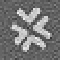
\includegraphics[height=\heightof{M}]{autanet.pdf}}
\definecolor{mygray}{gray}{0.333}
\iftypodisclaim%
\ifafour\newcommand\addprintnote{\begin{picture}(0,0)%
\put(245,149){\makebox(0,0){\rotatebox{90}{\tiny\color{mygray}\textsf{This
            document is designed for screen reading and
            two-up printing on A4 or Letter paper}}}}%
\end{picture}}% A4
\else\newcommand\addprintnote{\begin{picture}(0,0)%
\put(176,112){\makebox(0,0){\rotatebox{90}{\tiny\color{mygray}\textsf{This
            document is designed for screen reading and
            two-up printing on A4 or Letter paper}}}}%
\end{picture}}\fi%afourtrue
\makeoddfoot{plain}{}{\makebox[0pt]{\thepage}\addprintnote}{}
\else
\makeoddfoot{plain}{}{\makebox[0pt]{\thepage}}{}
\fi%typodisclaimtrue
\makeoddhead{plain}{\footnotesize\reporthead}{}{}

% \copypagestyle{manainitial}{plain}
% \makeheadrule{manainitial}{\headwidth}{0.5\normalrulethickness}
% \makeoddhead{manainitial}{%
% \footnotesize\sffamily%
% \scshape\headauthor}{}{\footnotesize\sffamily%
% \headtitle}
% \makeoddfoot{manaart}{}{\thepage}{}

\pagestyle{manaart}

\setlength{\droptitle}{-3.9\onelineskip}
\pretitle{\begin{center}\LARGE\sffamily%
\bfseries}
\posttitle{\bigskip\end{center}}

\makeatletter\newcommand*{\atf}{
\includegraphics[%trim=1pt 1pt 0pt 0pt,
totalheight=\heightof{@}]{atblack.png}}\makeatother
\providecommand{\affiliation}[1]{\textsl{\textsf{\footnotesize #1}}}
\providecommand{\epost}[1]{\texttt{\footnotesize\textless#1\textgreater}}
\providecommand{\email}[2]{\href{mailto:#1ZZ@#2 ((remove ZZ))}{#1\protect\atf#2}}

\preauthor{\vspace{-0.5\baselineskip}\begin{center}
\normalsize\sffamily%
\lineskip  0.5em}
\postauthor{\par\end{center}}
\predate{\DTMsetdatestyle{mydate}\begin{center}\footnotesize}
\postdate{\end{center}\vspace{-\medskipamount}}
\usepackage[british]{datetime2}
\DTMnewdatestyle{mydate}%
{% definitions
\renewcommand*{\DTMdisplaydate}[4]{%
\number##3\ \DTMenglishmonthname{##2} ##1}%
\renewcommand*{\DTMDisplaydate}{\DTMdisplaydate}%
}
\DTMsetdatestyle{mydate}


\setfloatadjustment{figure}{\footnotesize}
\captiondelim{\quad}
\captionnamefont{\footnotesize\sffamily%
}
\captiontitlefont{\footnotesize}
\firmlists*
\midsloppy

% handling orphan/widow lines, memman.pdf
% \clubpenalty=10000
% \widowpenalty=10000
% \raggedbottom
% Downes, memman.pdf
\clubpenalty=9996
\widowpenalty=9999
\brokenpenalty=4991
\predisplaypenalty=10000
\postdisplaypenalty=1549
\displaywidowpenalty=1602

\selectlanguage{british}\frenchspacing
%%%%%%%%%%%%%%%%%%%%%%%%%%%%%%%%%%%%%%%%%%%%%%%%%%%%%%%%%%%%%%%%%%%%%%%%%%%%
%%%%%%%%%%%%%%%%%%%%%%%%%%%%%%%%%%%%%%%%%%%%%%%%%%%%%%%%%%%%%%%%%%%%%%%%%%%%
%%%% Paper's details %%%%
\title{\propertitle%\\
%  {\large A geometric commentary on maximum-entropy proofs}% ***
}
\author{% 
\hspace*{\stretch{1}}%
\parbox{0.5\linewidth}%\makebox[0pt][c]%
{\protect\centering P.G.L. Porta\,Mana\\%
\footnotesize\epost{\email{piero.mana}{ntnu.no}}}%
\hspace*{\stretch{1}}%
\parbox{0.5\linewidth}%
{\protect\centering Y. Roudi\\%
\footnotesize\epost{\email{yasser.roudi}{ntnu.no}}}%
\hspace*{\stretch{1}}%
%\quad\href{https://orcid.org/0000-0002-6070-0784}{\protect
\includegraphics[scale=0.16]{orcid_32x32.png}\textsc{orcid}:0000-0002-6070-0784}%
}

%\date{Draft of \today\ (first drafted \firstdraft)}
%\date{\firstpublished; updated \updated}
\date{\firstdraft; updated \updated}

%@@@@@@@@@@ new macros @@@@@@@@@@
% Common ones - uncomment as needed
%\providecommand{\nequiv}{\not\equiv}
%\providecommand{\coloneqq}{\mathrel{\mathop:}=}
%\providecommand{\eqqcolon}{=\mathrel{\mathop:}}
%\providecommand{\varprod}{\prod}
\newcommand*{\de}{\partialup}%partial diff
\newcommand*{\pu}{\piup}%constant pi
\newcommand*{\delt}{\deltaup}%Kronecker, Dirac
%\newcommand*{\eps}{\varepsilonup}%Levi-Civita, Heaviside
%\newcommand*{\riem}{\zetaup}%Riemann zeta
%\providecommand{\degree}{\textdegree}% degree
%\newcommand*{\celsius}{\textcelsius}% degree Celsius
%\newcommand*{\micro}{\textmu}% degree Celsius
%\newcommand*{\I}{\mathrm{i}}%imaginary unit
%\newcommand*{\e}{\mathrm{e}}%Neper
\newcommand*{\di}{\mathrm{d}}%differential
%\newcommand*{\Di}{\mathrm{D}}%capital differential
%\newcommand*{\planckc}{\hslash}
%\newcommand*{\avogn}{N_{\textrm{A}}}
%\newcommand*{\NN}{\bm{\mathrm{N}}}
%\newcommand*{\ZZ}{\bm{\mathrm{Z}}}
%\newcommand*{\QQ}{\bm{\mathrm{Q}}}
\newcommand*{\RR}{\bm{\mathrm{R}}}
\newcommand*{\CC}{\bm{\mathrm{C}}}
%\newcommand*{\nabl}{\bm{\nabla}}%nabla
%\DeclareMathOperator{\lb}{lb}%base 2 log
%\DeclareMathOperator{\tr}{tr}%trace
%\DeclareMathOperator{\card}{card}%cardinality
%\DeclareMathOperator{\im}{Im}%im part
%\DeclareMathOperator{\re}{Re}%re part
%\DeclareMathOperator{\sgn}{sgn}%signum
%\DeclareMathOperator{\ent}{ent}%integer less or equal to
%\DeclareMathOperator{\Ord}{O}%same order as
%\DeclareMathOperator{\ord}{o}%lower order than
%\newcommand*{\incr}{\triangle}%finite increment
\newcommand*{\defd}{\coloneqq}
\newcommand*{\defs}{\eqqcolon}
%\newcommand*{\Land}{\bigwedge}
%\newcommand*{\Lor}{\bigvee}
%\newcommand*{\lland}{\mathbin{\ \land\ }}
%\newcommand*{\llor}{\mathbin{\ \lor\ }}
%\newcommand*{\lonlyif}{\mathbin{\Rightarrow}}%implies
%\newcommand*{\limplies}{\mathbin{\Rightarrow}}%implies
\newcommand*{\mimplies}{\Rightarrow}%implies
%\newcommand*{\liff}{\mathbin{\Leftrightarrow}}%if and only if
%\newcommand*{\cond}{\mathpunct{|}}%conditional sign (in probabilities)
%\newcommand*{\lcond}{\mathpunct{|\ }}%conditional sign (in probabilities)
%\newcommand*{\bigcond}{\mathpunct{\big|}}%conditional sign (in probabilities)
%\newcommand*{\lbigcond}{\mathpunct{\big|\ }}%conditional sign (in probabilities)
\newcommand*{\suchthat}{\mid}%{\mathpunct{|}}%such that (eg in sets)
%\newcommand*{\bigst}{\mathpunct{\big|}}%such that (eg in sets)
%\newcommand*{\with}{\colon}%with (list of indices)
%\newcommand*{\mul}{\times}%multiplication
%\newcommand*{\inn}{\cdot}%inner product
%\newcommand*{\dotv}{\mathord{\,\cdot\,}}%variable place
%\newcommand*{\comp}{\circ}%composition of functions
%\newcommand*{\con}{\mathbin{:}}%scal prod of tensors
%\newcommand*{\equi}{\sim}%equivalent to 
\renewcommand*{\asymp}{\simeq}%equivalent to 
%\newcommand*{\corr}{\mathrel{\hat{=}}}%corresponds to
%\providecommand{\varparallel}{\ensuremath{\mathbin{/\mkern-7mu/}}}%parallel (tentative symbol)
\renewcommand{\le}{\leqslant}%less or equal
\renewcommand{\ge}{\geqslant}%greater or equal
\DeclarePairedDelimiter\clcl{[}{]}
\DeclarePairedDelimiter\clop{[}{[}
%\DeclarePairedDelimiter\opcl{]}{]}
%\DeclarePairedDelimiter\opop{]}{[}
%\DeclarePairedDelimiter\abs{\lvert}{\rvert}
%\DeclarePairedDelimiter\norm{\lVert}{\rVert}
\DeclarePairedDelimiter\set{\{}{\}}
%\DeclareMathOperator{\pr}{P}%probability
\newcommand*{\pf}{\mathrm{p}}%probability
\newcommand*{\p}{\mathrm{P}}%probability
%\newcommand*{\tf}{\mathrm{T}}%probability
\renewcommand*{\|}{\mathpunct{|}}
%\newcommand*{\lcond}{\mathpunct{|\ }}%conditional sign (in probabilities)
\newcommand*{\bigcond}{\mathpunct{\big|\ }}%conditional sign (in probabilities)
%\newcommand*{\lbigcond}{\mathpunct{\big|\ }}%conditional sign (in probabilities)
%\newcommand*{\+}{\lor}
%\renewcommand{\*}{\land}
\newcommand*{\sect}{\S}% Sect.~
\newcommand*{\sects}{\S\S}% Sect.~
\newcommand*{\chap}{ch.}%
\newcommand*{\chaps}{chs}%
\newcommand*{\bref}{ref.}%
\newcommand*{\brefs}{refs}%
%\newcommand*{\fn}{fn}%
\newcommand*{\eqn}{eq.}%
\newcommand*{\eqns}{eqs}%
\newcommand*{\fig}{fig.}%
\newcommand*{\figs}{figs}%
\newcommand*{\vs}{{vs}}
%\newcommand*{\etc}{{etc.}}
%\newcommand*{\ie}{{i.e.}}
%\newcommand*{\ca}{{c.}}
%\newcommand*{\eg}{{e.g.}}
\newcommand*{\foll}{{ff.}}
%\newcommand*{\viz}{{viz}}
\newcommand*{\cf}{{cf.}}
%\newcommand*{\Cf}{{Cf.}}
%\newcommand*{\vd}{{v.}}
\newcommand*{\etal}{{et al.}}
%\newcommand*{\etsim}{{et sim.}}
%\newcommand*{\ibid}{{ibid.}}
%\newcommand*{\sic}{{sic}}
%\newcommand*{\id}{\mathte{I}}%id matrix
%\newcommand*{\nbd}{\nobreakdash}%
%\newcommand*{\bd}{\hspace{0pt}}%
%\def\hy{-\penalty0\hskip0pt\relax}
%\newcommand*{\labelbis}[1]{\tag*{(\ref{#1})$_\text{r}$}}
%\newcommand*{\mathbox}[2][.8]{\parbox[t]{#1\columnwidth}{#2}}
%\newcommand*{\zerob}[1]{\makebox[0pt][l]{#1}}
\newcommand*{\tprod}{\mathop{\textstyle\prod}\nolimits}
\newcommand*{\tsum}{\mathop{\textstyle\sum}\nolimits}
%\newcommand*{\tint}{\begingroup\textstyle\int\endgroup\nolimits}
%\newcommand*{\tland}{\mathop{\textstyle\bigwedge}\nolimits}
%\newcommand*{\tlor}{\mathop{\textstyle\bigvee}\nolimits}
%\newcommand*{\sprod}{\mathop{\textstyle\prod}}
%\newcommand*{\ssum}{\mathop{\textstyle\sum}}
%\newcommand*{\sint}{\begingroup\textstyle\int\endgroup}
%\newcommand*{\sland}{\mathop{\textstyle\bigwedge}}
%\newcommand*{\slor}{\mathop{\textstyle\bigvee}}
\newcommand*{\T}{^\intercal}%transpose
\newcommand*{\E}{\mathrm{E}}
\DeclarePairedDelimiter\expp{(}{)}
\newcommand*{\expe}{\E\expp}%round
\newcommand*{\expeb}{\E\clcl}%square
%%\newcommand*{\QEM}%{\textnormal{$\Box$}}%{\ding{167}}
%\newcommand*{\qem}{\leavevmode\unskip\penalty9999 \hbox{}\nobreak\hfill
%\quad\hbox{\QEM}}

\definecolor{notecolour}{RGB}{68,170,153}
%\newcommand*{\puzzle}{{\fontencoding{U}\fontfamily{fontawesometwo}\selectfont\symbol{225}}}
\newcommand*{\puzzle}{\maltese}
\newcommand{\mynote}[1]{ {\color{notecolour}\puzzle\ #1}}
\newcommand*{\widebar}[1]{{\mkern1.5mu\skew{2}\overline{\mkern-1.5mu#1\mkern-1.5mu}\mkern 1.5mu}}

\DeclareMathOperator*{\argsup}{arg\,sup}
\newcommand*{\yI}{\varIota}
\newcommand*{\ys}{\bm{s}}
\newcommand*{\yH}{\varEta}
\newcommand*{\yD}{D}
\newcommand*{\yA}{\varAlpha}
\newcommand*{\yso}[1]{\ys^{(#1)}}
\newcommand*{\ysso}[1]{s^{(#1)}}
\newcommand*{\la}{\mu_{12}}
\newcommand*{\yth}{\bm{\mu}}
\newcommand*{\ythm}{\yth_{\text{m}}}
\newcommand*{\yt}{\bm{m}}
\newcommand*{\yl}{m_{12}}
\newcommand*{\yq}{\bm{q}}
\newcommand*{\yql}{q_{3}}
\newcommand*{\yav}{\widebar{\ys}}
\newcommand*{\yavv}{\widebar{s}}
\newcommand*{\ycv}{\widebar{ss}}
\newcommand*{\ym}{\bm{m}}
\newcommand*{\V}{\mathrm{V}}
\newcommand*{\var}{\V\expp}%round
\newcommand*{\varb}{\V\clcl}%square
\newcommand*{\yIth}{\yI_{\yth}}
\newcommand*{\yIt}{\yI_{\yt}}
\newcommand*{\yN}{\varLambda}
\newcommand*{\ynn}{\nu}
\newcommand*{\yn}{\bm{\nu}}
\newcommand*{\simpl}{\varDelta}
\newcommand*{\yff}{f}
\newcommand*{\yf}{\bm{\yff}}
%@@@@@@@@@@ new macros end @@@@@@@@@@

\firmlists
\begin{document}
\captiondelim{\quad}\captionnamefont{\footnotesize}\captiontitlefont{\footnotesize}
\selectlanguage{british}\frenchspacing

%%% Title and abstract %%%
\maketitle
\ifpublic
\abstractrunin
\abslabeldelim{}
\renewcommand*{\abstractname}{}
\setlength{\absleftindent}{0pt}
\setlength{\absrightindent}{0pt}
\setlength{\abstitleskip}{-\absparindent}
\begin{abstract}\labelsep 0pt%
  \noindent Study of uniform priors in parameter space and in constraint
  space for Ising models
% \par%\\[\jot]
% \noindent
% {\footnotesize PACS: ***}\qquad%
% {\footnotesize MSC: ***}%
%\qquad{\footnotesize Keywords: ***}
\end{abstract}\fi

\selectlanguage{british}\frenchspacing
% \asudedication{\small ***}
% \vspace{\bigskipamount}

\setlength{\epigraphwidth}{.63\columnwidth}
% %\epigraphposition{flushright}
\epigraphtextposition{flushright}
% %\epigraphsourceposition{flushright}
\epigraphfontsize{\footnotesize}
\setlength{\epigraphrule}{0pt}
% %\setlength{\beforeepigraphskip}{0pt}
% %\setlength{\afterepigraphskip}{0pt}
\epigraph{\enquote{Flat priors do not exist}}{(anonymous)}

\iffalse\noindent\emph{\footnotesize Note: Dear Peer, this manuscript is
  peer-reviewed by \emph{you}. I'm grateful if you let me know of any
  faults in its premisses, logic, evidence, and of any other criticisms you
  may have.}
\fi

\section{Initial assumptions for models with second-order sufficient
  statistics}
\label{sec:2_suff_stat}

\subsection{A two-unit model with sufficient statistics}
\label{sec:intro}

Consider a population consisting in two binary units $\ys \defd (s_1,s_2)$
with values in $\set{0,1}$. One observation of this population can give
four results: $\ys \in \set{00,01,10,11}$.

We have $N$ observations $(\yso{1}, \dotsc, \yso{N})$ of this or other
populations prepared in similar conditions, so that knowledge of these
observations is relevant for our forecast of a new observation $\ys$, again
in similar conditions. We assume that only the number, the mean, and the
second moments of these past observations are relevant to forecast the new
one; that is, we have these sufficient statistics:
\begin{equation}
  \label{eq:mean_2ndmom}
  N,\quad
  \tfrac{1}{N}\bigl( \yso{1} + \dotsb + \yso{N} \bigr) \defs \yav,
  \quad
  \tfrac{1}{N}\bigl( \ysso{1}_1\ysso{1}_2 + \dotsb + \ysso{N}_1 \ysso{N}_2 \bigr)
  \defs \ycv
\end{equation}
These assumptions are collectively denoted $\yI$.

A series of mathematical results, which we call the
Koopman-Pitman-Lauritzen theorem, says that our probabilistic forecasts
must assume this general form, for any $N$:
\begin{multline}
  \label{eq:predictive_KP}
    \pf(\yso{1}, \dotsc, \yso{N} \|\yI )
\\  
\begin{aligned}
  &=\int
\Biggl[  \prod_{i=1}^{N}
  g\bigl(\yso{i}\bigr)\,
  \frac{  \exp\bigl(
    \mu_1\, \ysso{i}_1 + \mu_2\, \ysso{i}_2 + \la\, \ysso{i}_1 \ysso{i}_2
    \bigr) }{Z(\yth)}
  \Biggr]\,
  \pf(\yth \| \yI)\,\di\yth 
\\
  &=\int
  \bigl[\tprod_{i=1}^{N}g\bigl(\yso{i}\bigr) \bigr]\,
  \frac{  \exp[N \, (
    \mu_1\, \yavv_1 + \mu_2\, \yavv_2 + \la\, \ycv)]}{Z(\yth)^N}
\,  \pf(\yth \| \yI)\,\di\yth 
\end{aligned}
\\
\text{with}\quad
\yth\defd (\mu_1,\mu_2,\la) \in \RR^3,\\
  Z(\yth) \defd
  g(00)+ g(10)\,\exp(\mu_1) + g(01)\,\exp(\mu_2) + g(11)\,\exp(\mu_1+\mu_2+\la).
\end{multline}

The distribution $g(\ys)$ and the density $\pf(\yth \| \yI)\,\di\yth $ in
the formula above are not determined by the theorem: they need to be
determined by additional assumptions. The distribution $g$ is often
determined by symmetry or combinatorial properties of the problem.
% for example, if each unit actually represents the total activity of a
% population of sub-units.
From now on we assume it to be unity: $g(\ys)=1$. The density
$\pf(\yth \|\yI)\,\di\yth $ is called \emph{prior parameter density}.

The formula above says that our joint probability distribution for the $N$
outcomes is given by a mixture of joint, factorizable distributions from a
three-parameter family. This family is a submanifold in the space of all
possible joint distributions, which has dimension $4^N-1$. The parameters
$\yth$ are coordinates in this submanifold, each triplet identifying a
particular factorizable distribution
\begin{equation}
  \label{eq:extreme_distributions}
    \pf(\yso{1}, \dotsc, \yso{N} \|\yth, \yI ) =
  \prod_{i=1}^{N}
  \frac{  \exp\bigl(
    \mu_1\, \ysso{i}_1 + \mu_2\, \ysso{i}_2 + \la\, \ysso{i}_1 \ysso{i}_2
    \bigr) }{Z(\yth)}.
\end{equation}
The weights of the mixture are $\pf(\yth \|\yI)\,\di\yth $.

From the integral of the formula~\eqref{eq:predictive_KP} and the geometric
interpretation above it is clear that the theorem does not select the
coordinates $\yth$. We can choose another set of coordinates
$\yt \defd (m_1,m_2,\yl)$, related to the $\yth$ by a one-one
transformation $\yt(\yth)$ with inverse $\yth(\yt)$. The three-dimensional
family is then labelled as
\begin{equation}
  \label{eq:extreme_distributions_relabelled}
    \pf(\yso{1}, \dotsc, \yso{N} \|\yt, \yI ) =
  \prod_{i=1}^{N}
  \frac{  \exp\bigl[ 
    \mu_1(\yt)\, \ysso{i}_1 + \mu_2(\yt)\, \ysso{i}_2 +
    \la(\yt)\, \ysso{i}_1 \ysso{i}_2
    \bigr] }{Z[\yth(\yt)]},
\end{equation}
the prior parameter density is
\begin{equation}
  \label{eq:density_new_coords}
  \pf(\yt \|\yI)\,\di\yt  =
  \det\biggl( \frac{\de\yt}{\de\yth}\biggr)\, \pf(\yth \| \yI)\,\di\yth ,
\end{equation}
and the integral formula becomes, with $g(\ys)=1$,
\begin{multline}
  \label{eq:predictive_KP}
  \pf(\yso{1}, \dotsc, \yso{N} \|\yI )
  \\
\begin{aligned}
  &=\int
\Biggl[  \prod_{i=1}^{N}
  \frac{  \exp\bigl[ 
    \mu_1(\yt)\, \ysso{i}_1 + \mu_2(\yt)\, \ysso{i}_2 +
    \la(\yt)\, \ysso{i}_1 \ysso{i}_2
    \bigr] }{Z[\yth(\yt)]}
  \Biggr]\,
  \pf(\yt \| \yI)\,\di\yt 
\\
  &=\int
  \frac{  \exp\{N \, [
    \mu_1(\yt)\, \yavv_1 + \mu_2(\yt)\, \yavv_2 +
    \la(\yt)\, \ycv)]\}}{Z[\yth(\yt)]^N}
\,  \pf(\yt \| \yI)\,\di\yt ,
\end{aligned}
\end{multline}
equivalent to~\eqref{eq:predictive_KP}.

This coordinate change is central to the rest of this study.

\textcolor{white}{If you find this you can claim a postcard from me.}

\subsection{New coordinates and their motivation}
\label{sec:new_coords}

Assuming that~\eqref{eq:mean_2ndmom} are sufficient statistics and
therefore using formula~\eqref{eq:predictive_KP}, let's ask what's the
limit probability of observing particular values of the statistics $\yav$,
$\ycv$ for very large $N$; that is, $\pf(\yav,\ycv \| \yI, \text{large } N)$.

In this section we show that there is a particular coordinate system
$\yt \defd (m_1, m_2, \yl)$ of the three-dimensional manifold discussed above
for which \emph{the prior parameter density coincides, in the large-$N$
  limit, with the probability of the observed statistics}:
\begin{equation}
  \label{eq:special_parameter_is_statistics}
  \pf[(\yavv_1,\yavv_2,\ycv)=\bm{x} \| \yI, \text{large $N$}]
  \approx \pf(\yt=\bm{x} \|\yI).
\end{equation}

To see this, consider the parameterized, factorized joint probability
$\pf(\yso{1}, \dotsc, \yso{N} \|\yth, \yI )$ of
\eqn~\eqref{eq:component_combination}. The expectation of the statistics
$(\yavv_1,\yavv_2,\ycv)$ is given by
\begin{multline}
  \label{eq:expect_statistics}
  \expeb{(\yavv_1,\yavv_2,\ycv) \|\yth,\yI} ={}\\
  \tfrac{1}{N} \sum_{i}
  \expeb{(\ysso{i}_1,\ysso{i}_2,\ysso{i}_1 \ysso{i}_2) \|\yth,\yI}
  = \expeb{(s_1,s_2,s_1 s_2) \|\yth,\yI}
\end{multline}
where $(s_1,s_2,s_1 s_2)$ refer to any one of the $N$ observations. The two
equalities come from the properties of the expectation and the factorized
form of the joint probability conditional on $\yth$. From the properties of
the variance we also have
\begin{equation}
  \label{eq:variance_statistics}
  \varb{(\yavv_1,\yavv_2,\ycv) \|\yth,\yI}
  = \frac{1}{N} \varb{(s_1,s_2,s_1 s_2) \|\yth,\yI}.
\end{equation}

This means that for a triplet $\yth$, for large $N$ we have a probability
distribution for the statistics that is very peaked at particular values
$\yt \defd (m_1,m_2,\yl)$ determined by the equations
\begin{equation}
  \label{eq:change_coords}
  \begin{gathered}
    m_1 = \expe{s_1 \|\yth,\yI}
    \equiv \frac{\de\ln Z(\yth)}{\de \mu_1},
    \qquad
  m_2 = \expe{s_2 \|\yth,\yI}
    \equiv \frac{\de\ln Z(\yth)}{\de \mu_2},\\
  \yl = \expe{s_1 s_2\|\yth,\yI}
    \equiv \frac{\de\ln Z(\yth)}{\de\la}.
  \end{gathered}
\end{equation}
This system of equations actually puts the parameters
$\yth \defd(\mu_1, \mu_2, \la)$
and $\yt\defd(m_1, m_2,\yl)$ into one-one
correspondence \citep{meadetal1984}. The former belong to $\RR^3$; the
latter to the bounded domain
\begin{equation}
  \label{eq:domain_newcoords}
  0\le m_1,m_2 \le 1,
  \qquad
  \max(0,m_1 + m_2 -1) \le \yl \le \min(m_1,m_2)
\end{equation}
shown in \fig~\ref{fig:domain}.
%\setlength{\intextsep}{0.5ex}% with wrapfigure
\begin{figure}%{r}{0.4\linewidth} % with wrapfigure
  \centering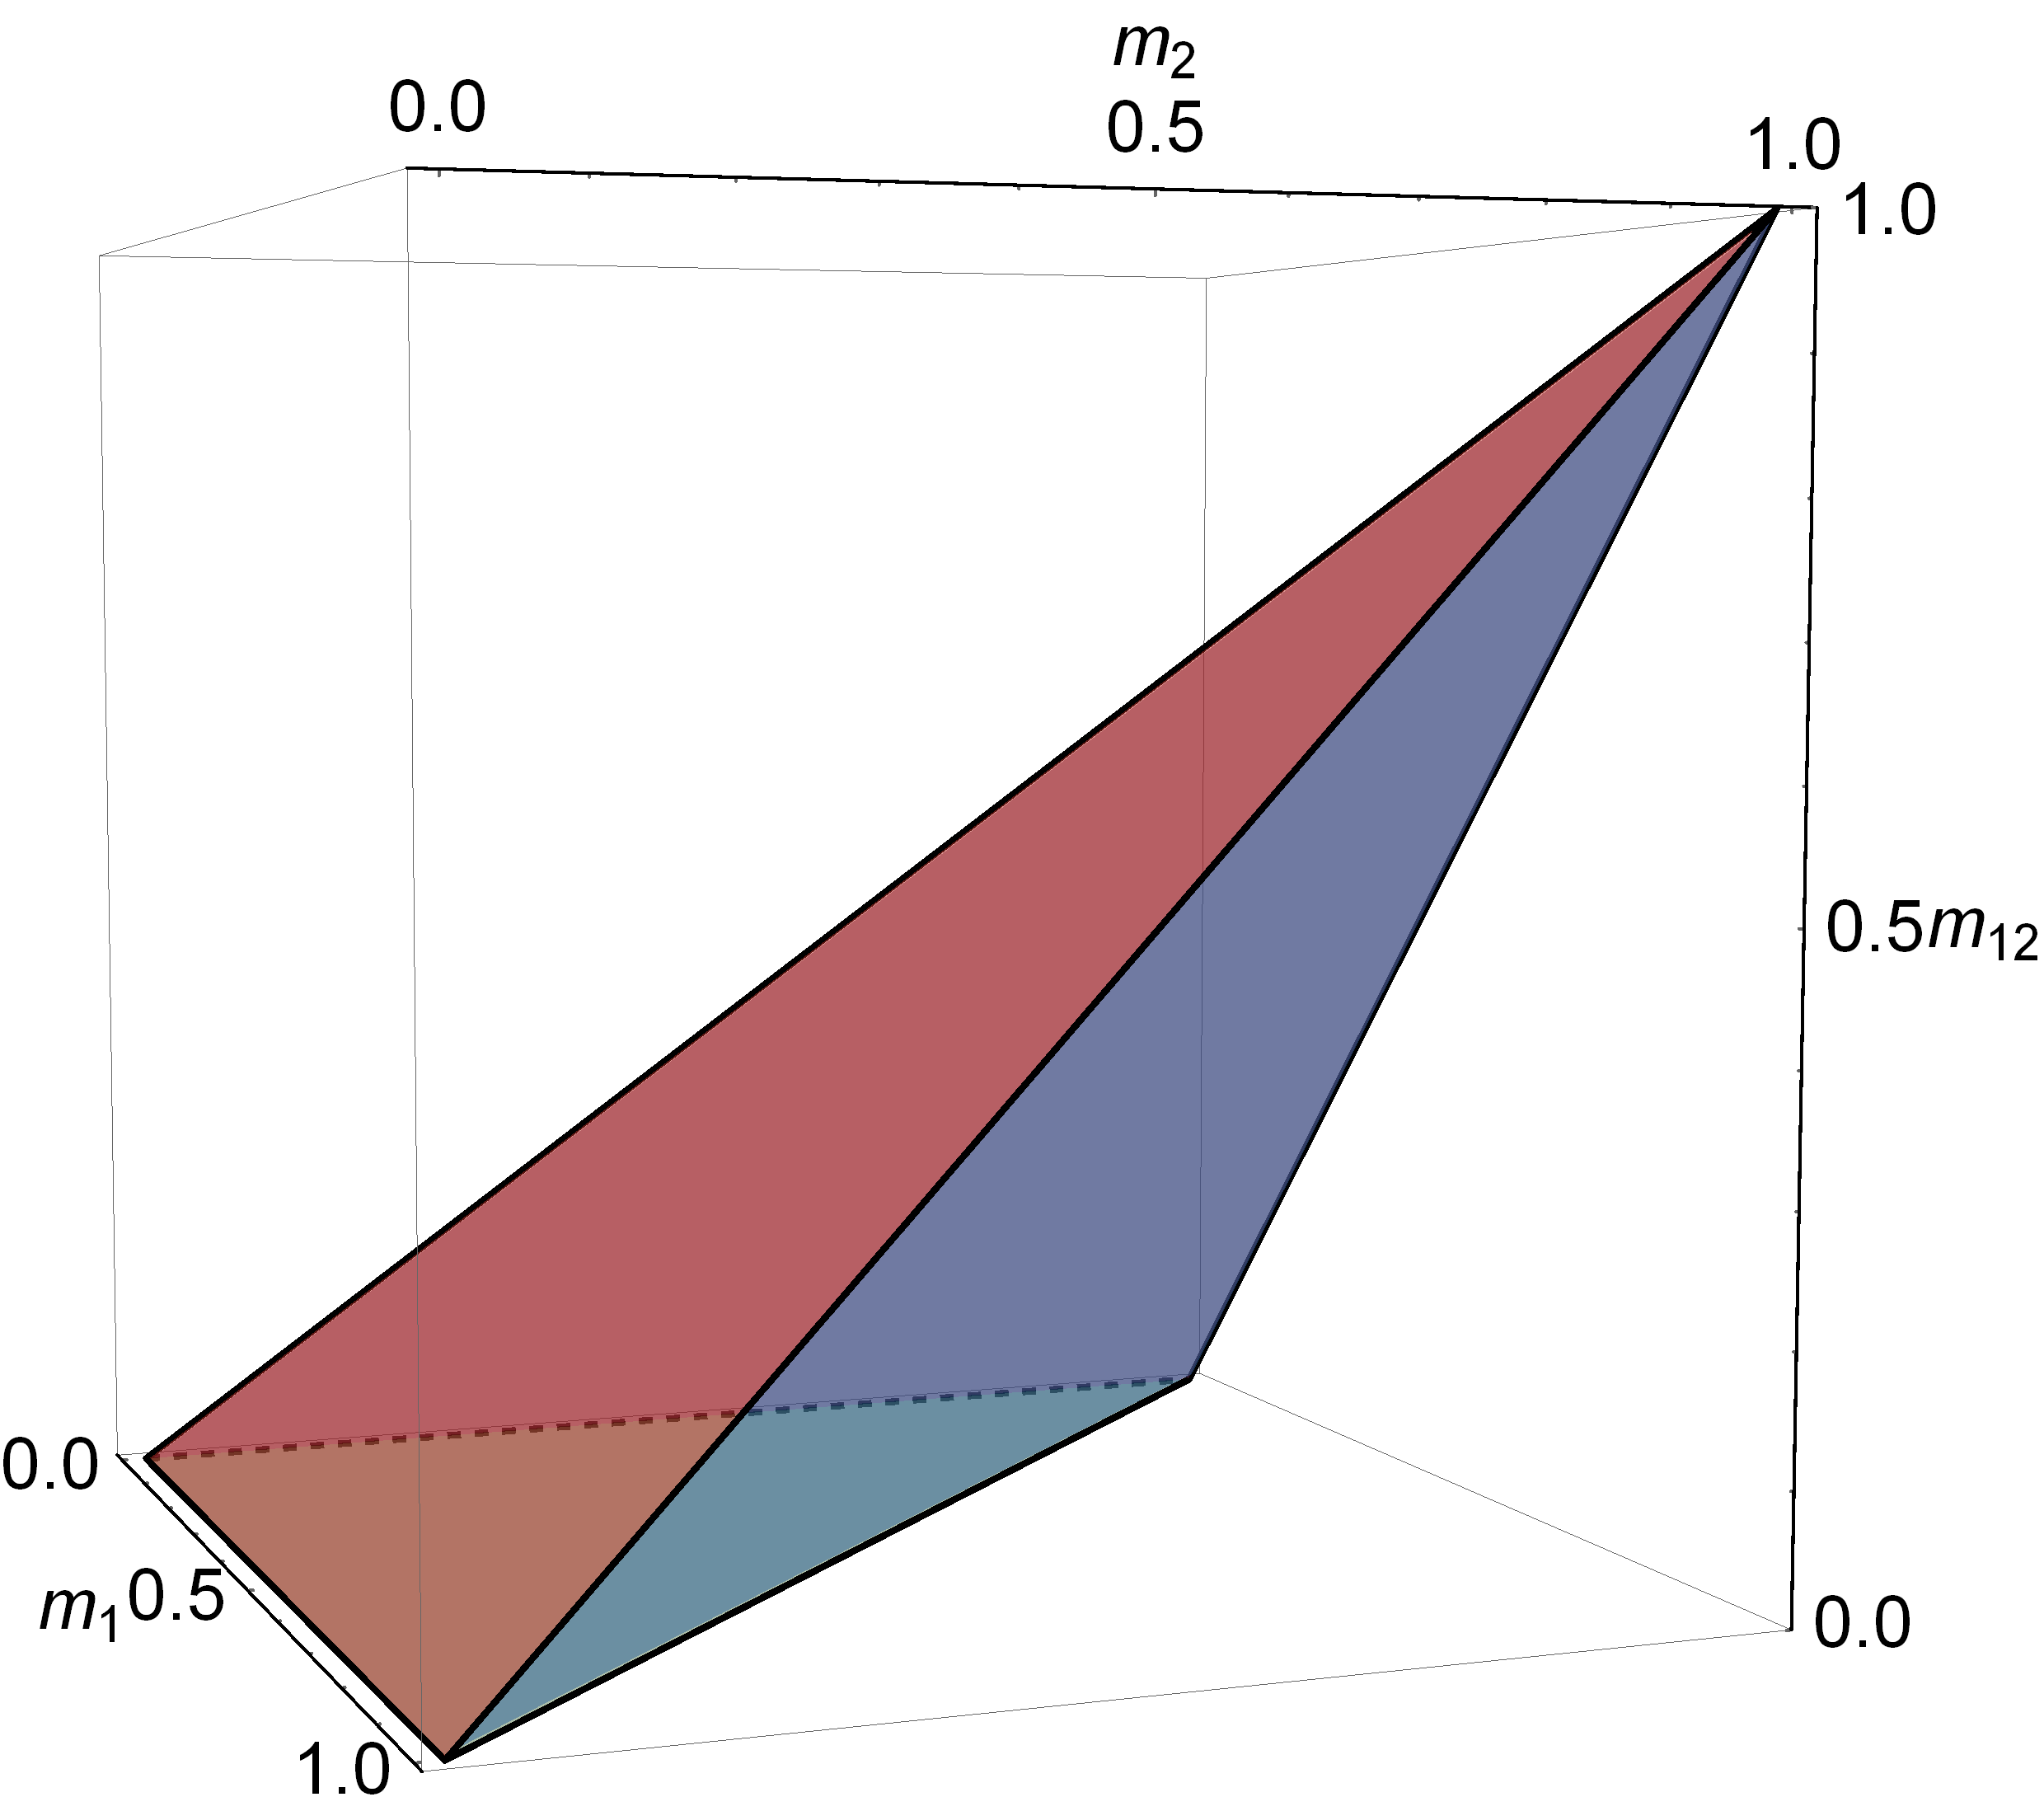
\includegraphics[width=0.75\linewidth]{domain.png}\\
  \caption{}
  \label{fig:domain}
\end{figure}% dimer_study.nb

Using these new parameters, the probability for statistics $(\yav,\ycv)$
becomes for large $N$
\begin{equation}
  \label{eq:prob_stat_newparams}
  \pf(\yavv_1,\yavv_2,\ycv \|m_1,m_2,\yl,\yI)
  \approx \delt[(\yavv_1,\yavv_2,\ycv)- (m_1, m_2, \yl)].
\end{equation}
Taking the convex combination of this expression in $\yt$ with weights
$\pf(\yt \|\yI)\,\di\yt$ we obtain
\eqn~\eqref{eq:special_parameter_is_statistics}.

\bigskip

In the coordinates $\yt$, the formula~\eqref{eq:predictive_KP} given
by the theorem can be interpreted in the following way.
\begin{enumerate}%[label=(\textit{\arabic*})]
\item We first assume to know that the limit statistics in a very large
  number of observations is $\yt \defd (m_1, m_2, \yl)$. Given this knowledge
  we can combinatorially calculate the probability of observing a finite
  sequence of $N$ observations, $\pf(\yso{1}, \dotsc, \yso{N} \|\yt,\yI)$,
  assuming that all sequences having given statistics are equally likely --
  this equiprobability corresponds to setting $g(\ys)=1$ in
  \eqn~\eqref{eq:predictive_KP}. An example of this combinatorial
  calculation is given below.
\item We then express our uncertainty about the limit statistics with the
  probability density $\pf(\yt \| \yI)\,\di\yt$.
\item The two uncertainties above are finally combined in the usual way
  using the law of total probability.
\end{enumerate}

\smallskip

Let's show, in the simplest case, that the probability conditional on
the statistics $\yt$,
\begin{equation}
  \label{eq:component_combination}
  \pf(\ys \|\yt, \yI )
  =
  % g\bigl(\yso{i}\bigr)\,
  \frac{  \exp\bigl[
    \mu_1(\yt)\, s_1 + \mu_2(\yt)\, s_2 + \la(\yt)\, s_1 s_2
    \bigr] }{Z[\yth(\yt)]}
\end{equation}
is indeed given combinatorially assuming equiprobability of all sequences,
as claimed above. Suppose that we know the limit statistics are
$(m_1, m_2, \yl)$. Only the outcome $\ys=11$ gives a non-vanishing
contribution to the second moment $\yl$, \eqn~\eqref{eq:mean_2ndmom}. This
number is therefore equal to the limit relative frequency of $11$. Assuming
equiprobability we set the probability of this outcome in the next
observation equal to this frequency $\yl$. Only the outcomes $10$ and $11$
give non-vanishing contributions to the mean $m_1$; this number is
therefore equal to their joint limit relative frequencies. Since the
frequency of $11$ is given by $\yl$, the frequency of $10$ must be given by
$m_1-\yl$, which is then our probability for this outcome in the next
observation. Analogous reasoning holds for the outcome $01$. Finally, the
limit relative frequencies of all four outcomes must sum to $1$; thus the
limit frequency and probability of outcome $00$ must be
$1-\yl-(m_1-1)-(m_2-\yl)$. Summarizing,
\begin{multline}
  \label{eq:prob_outcome_from_statistics}
  \pf(\ys \| \yt,\yI) =
  \begin{cases}
    1-m_1-m_2+\yl &\text{for } \ys=00\\
    m_1-\yl &\text{for } \ys=10\\
    m_2-\yl &\text{for } \ys=01\\
    \yl &\text{for } \ys=11
  \end{cases}
  \\[\jot]
  {}\equiv
    \yl^{s_1 s_2}\,
  (m_1-\yl)^{s_1-s_1 s_2}\,
  (m_2-\yl)^{s_2-s_1 s_2}\,
  (1-m_1-m_2+\yl)^{1-s_1-s_2+s_1 s_2}.
\end{multline}
This probability distribution is exactly
\eqn~\eqref{eq:component_combination}, as can be checked by finding
$\yth(\yt)$ with the inverse of the coordinate
transformations~\eqref{eq:change_coords},
\begin{equation}
  \label{eq:inverse_tranf_coord}
  \begin{gathered}
    \mu_1 =\ln\frac{m_1-\yl}{1+\yl-m_1-m_2},\qquad
    \mu_2 =\ln\frac{m_2-\yl}{1+\yl-m_1-m_2},\\[\jot]
\la =\ln\frac{(1+\yl-m_1-m_2)\,\yl}{(m_1-\yl)\,(m_2-\yl)},
\end{gathered}
\end{equation}
and substituting it in the right side of
\eqn~\eqref{eq:component_combination}.

\subsection{Scientifically motivated prior parameter densities}
\label{sec:other_priors}

The interpretation of the Koopman-Pitman-Lauritzen
formula~\eqref{eq:predictive_KP} explained in the previous section gives us
more intuitive grounds to choose the prior parameter density
$\pf(\yt \|\yI)\,\di\yt$: given the interpretation of the observables $\ys$
in a particular scientific context, which limit statistics $\yt$ would we
expect to observe?

If $\ys$ represents the binned activity of a neural population in the
brain, for example, from our research experience we consider more likely to
find low mean values $\yavv_1=m_1$, $\yavv_2=m_2$ than high ones, close to
$1$. We may also have some vague expectations about the second moments
$\ycv=\yl$. Even vague prior knowledge can be expressed by a probability
density with particular features, and this leads to better predictions.
Let's examine this possibility more concretely.

\bigskip


Using Bayes's theorem with formula~\eqref{eq:predictive_KP} we find our
probability for a new outcome $\ys$ conditional on observations
$\bigl( \yso{1}, \dotsc,\yso{N} \bigr)$:
\begin{subequations}    \label{eq:conditional_prediction}
  \begin{gather}
    \begin{multlined}[][0.9\linewidth]
      \pf(\ys \| \yso{1}, \dotsc, \yso{N}, \yI ) ={}\\[\jot]
      \int
      \frac{  \exp\bigl(
        \mu_1 s_1 + \mu_2 s_2 + \la s_1 s_2
        \bigr) }{Z(\yth)}
      \,
      % \times{}\\ \shoveright{
      \pf(\yth \| \yso{1},\dotsc,\yso{N} \yI) \, \di\yth
      % }
    \end{multlined}
    \\
    \shortintertext{with}
    \begin{multlined}[0.95\linewidth]
    \pf(\yth \| \yso{1},\dotsc,\yso{N} \yI)
    \propto
    \Biggl[  \prod_{i=1}^{N}
    \frac{  \exp\bigl(
      \mu_1 \ysso{i}_1 + \mu_2 \ysso{i}_2 + \la \ysso{i}_1 \ysso{i}_2
      \bigr) }{Z(\yth)}
    \Biggr]\,
    \pf(\yth \| \yI) 
\equiv{}\\[\jot]
     \exp\{N\,[
      \mu_1 a_1 + \mu_2 a_2 + \la \ycv -\ln Z(\yth)]\}\,
    \pf(\yth \| \yI).
  \end{multlined}
      \label{eq:posterior_density}
  \end{gather}
\end{subequations}
The density $\pf(\yth \| \yso{1},\dotsc,\yso{N} \yI)$ is called
\emph{posterior parameter density}.

The last expression shows that the $N$ observations affect our forecast
only through the averages $\yav$ and $\ycv$, \eqn~\eqref{eq:mean_2ndmom},
as we assumed.

The proportionality relation of the last formula reminds us that we must
perform an integral over $\yth$ to calculate the posterior parameter
density. We must also perform an integral over $\yth$ to calculate the
conditional probability for $\ys$. These integrals are difficult when we
consider populations with many units. When the number $N$ of known
observations is large, the posterior parameter density is often
approximated by a Dirac delta centred on the maximum of the posterior,
\begin{equation}
  \label{eq:max_posterior}
  \ythm \defd \argsup_{\yth}
  \{N\,[\mu_1 a_1 + \mu_2 a_2 + \la \ycv -\ln Z(\yth)]+
  \ln \pf(\yth \|\yI) \}.
\end{equation}
The probability for $\ys$ then equals the exponential calculated at
$\ythm$. If the prior parameter density $\pf(\yth \|\yI)$ is constant or
very broad, it can be dropped in the calculation of the maximum, as an
approximation.

The literature indeed often assumes a prior parameter density $\pf(\yth \|\yI)$
that is constant in $\yth$. This is an \enquote{improper}, non-normalizable
prior, because $\yth \in \RR^3$. So we are properly considering a
\emph{sequence} of normalizable priors of increasing width -- for example,
normal distributions with increasing variance -- and the resulting limit if
it exists.

How reasonable is prior density constant in $\yt$? Let's find the
equivalent density for the parameters $\yt$ discussed in the previous
section.

The Jacobian determinants of the transformations $\yth(\yt)$ and $\yt(\yth)$, from
\eqns~\eqref{eq:inverse_tranf_coord} and~\eqref{eq:change_coords}, are
\begin{subequations}  \label{eq:jacobian_transf}
  \begin{align}
    \det\biggl( \frac{\de\yth}{\de\yt}\biggr)
    &= \frac{1}{\yl\,(m_1-\yl)\,(m_2-\yl)\,(1+\yl-m_1-m_2)},
    \\
    \det\biggl( \frac{\de\yt}{\de\yth}\biggr)
    &=
\det\frac{\de^2\ln Z(\yth)}{\de\yth\,\de\yth}
=
      \frac{\exp(2\mu_1 + 2\mu_2 + \la)}{Z(\yth)^4}.
  \end{align}
\end{subequations}
These expressions are worthy of notice, because they can be uniquely written
as
\begin{subequations}    \label{eq:jacobian_as_probs}
  \begin{align}
    \det\biggl( \frac{\de\yth}{\de\yt}\biggr)
    &\!\!
      \begin{multlined}[t][0.85\linewidth]
=\frac{1}{
      \pf(00 \|\yt,\yI)\,
      \pf(10 \|\yt,\yI)\,
      \pf(01 \|\yt,\yI)\,
      \pf(11 \|\yt,\yI)}
      \equiv{}\\ \frac{1}{\prod_{\ys}\pf(\ys \|\yt,\yI)},
    \end{multlined}
      \\
      \det\biggl( \frac{\de\yt}{\de\yth}\biggr)
    &=
      \pf(00 \|\yth,\yI)\,
      \pf(10 \|\yth,\yI)\,
      \pf(01 \|\yth,\yI)\,
      \pf(11 \|\yth,\yI)
      \equiv \prod_{\ys}\pf(\ys \|\yth,\yI),
  \end{align}
\end{subequations}
as can be checked from \eqn~\eqref{eq:component_combination} for $N=1$.

Consider an assumption, denoted $\yIth$, that lead us to assign a constant
prior parameter density function $\pf(\yth \|\yIth)$. For $\yt$ such an
assumption corresponds to the density
\begin{multline}
  \label{eq:flat_density_in_statistics_space}
  \pf(\yt \|\yIth)\,\di\yt \propto
  \det\biggl( \frac{\de\yth}{\de\yt}\biggr)\,\di\yt
  \equiv{}\\
%  \frac{1}{\prod_{\ys}\pf(\ys \|\yt,\yI)}
%  \equiv{}\\
  \frac{\di\yt}{\yl\,(m_1-\yl)\,(m_2-\yl)\,(1+\yl-m_1-m_2)},
\end{multline}
obtained from \eqns~\eqref{eq:jacobian_as_probs}
and~\eqref{eq:prob_outcome_from_statistics}. This density, besides being
improper, gives very high probability to the extreme values of all three
statistics. It doesn't seem much appropriate in the context of brain
activity discussed above, for example.

Thus two questions appear: What densities are more appropriate? Do they
lead to more difficult computations than those used at present?

\bigskip

A simple parameter density that is normalizable and doesn't give too high
probability to extreme values of the statistics is that constant in the
$\yt$ coordinates; denote this assumption by $\yIt$:
\begin{equation}
  \label{eq:density_constant_statistics}
  \pf(\yt \| \yIt)\,\di\yt = 6\, \di\yt,
\end{equation}
the normalization constant calculated from solid geometry looking at the
pyramid of \fig~\ref{fig:domain}, having volume $1/6$. In terms of $\yth$
coordinates, using the Jacobian determinant~\eqref{eq:jacobian_as_probs},
it is
\begin{equation}
  \label{eq:density_constant_statistics_first_coords}
  \pf(\yth \|\yIt)\,\di\yth =
  6\,\biggl[ \prod_{\ys}\pf(\ys \|\yth,\yIt) \biggr]\,\di\yth
  \equiv
6\,  \frac{\exp(2\mu_1 + 2\mu_2 + \la)}{Z(\yth)^4}\,\di\yth.
\end{equation}
Its marginal for $(\mu_1,\la)$ is shown in
\fig~\ref{fig:marginal_flatstat}.
\begin{figure}[t!]%{r}{0.4\linewidth} % with wrapfigure
  \centering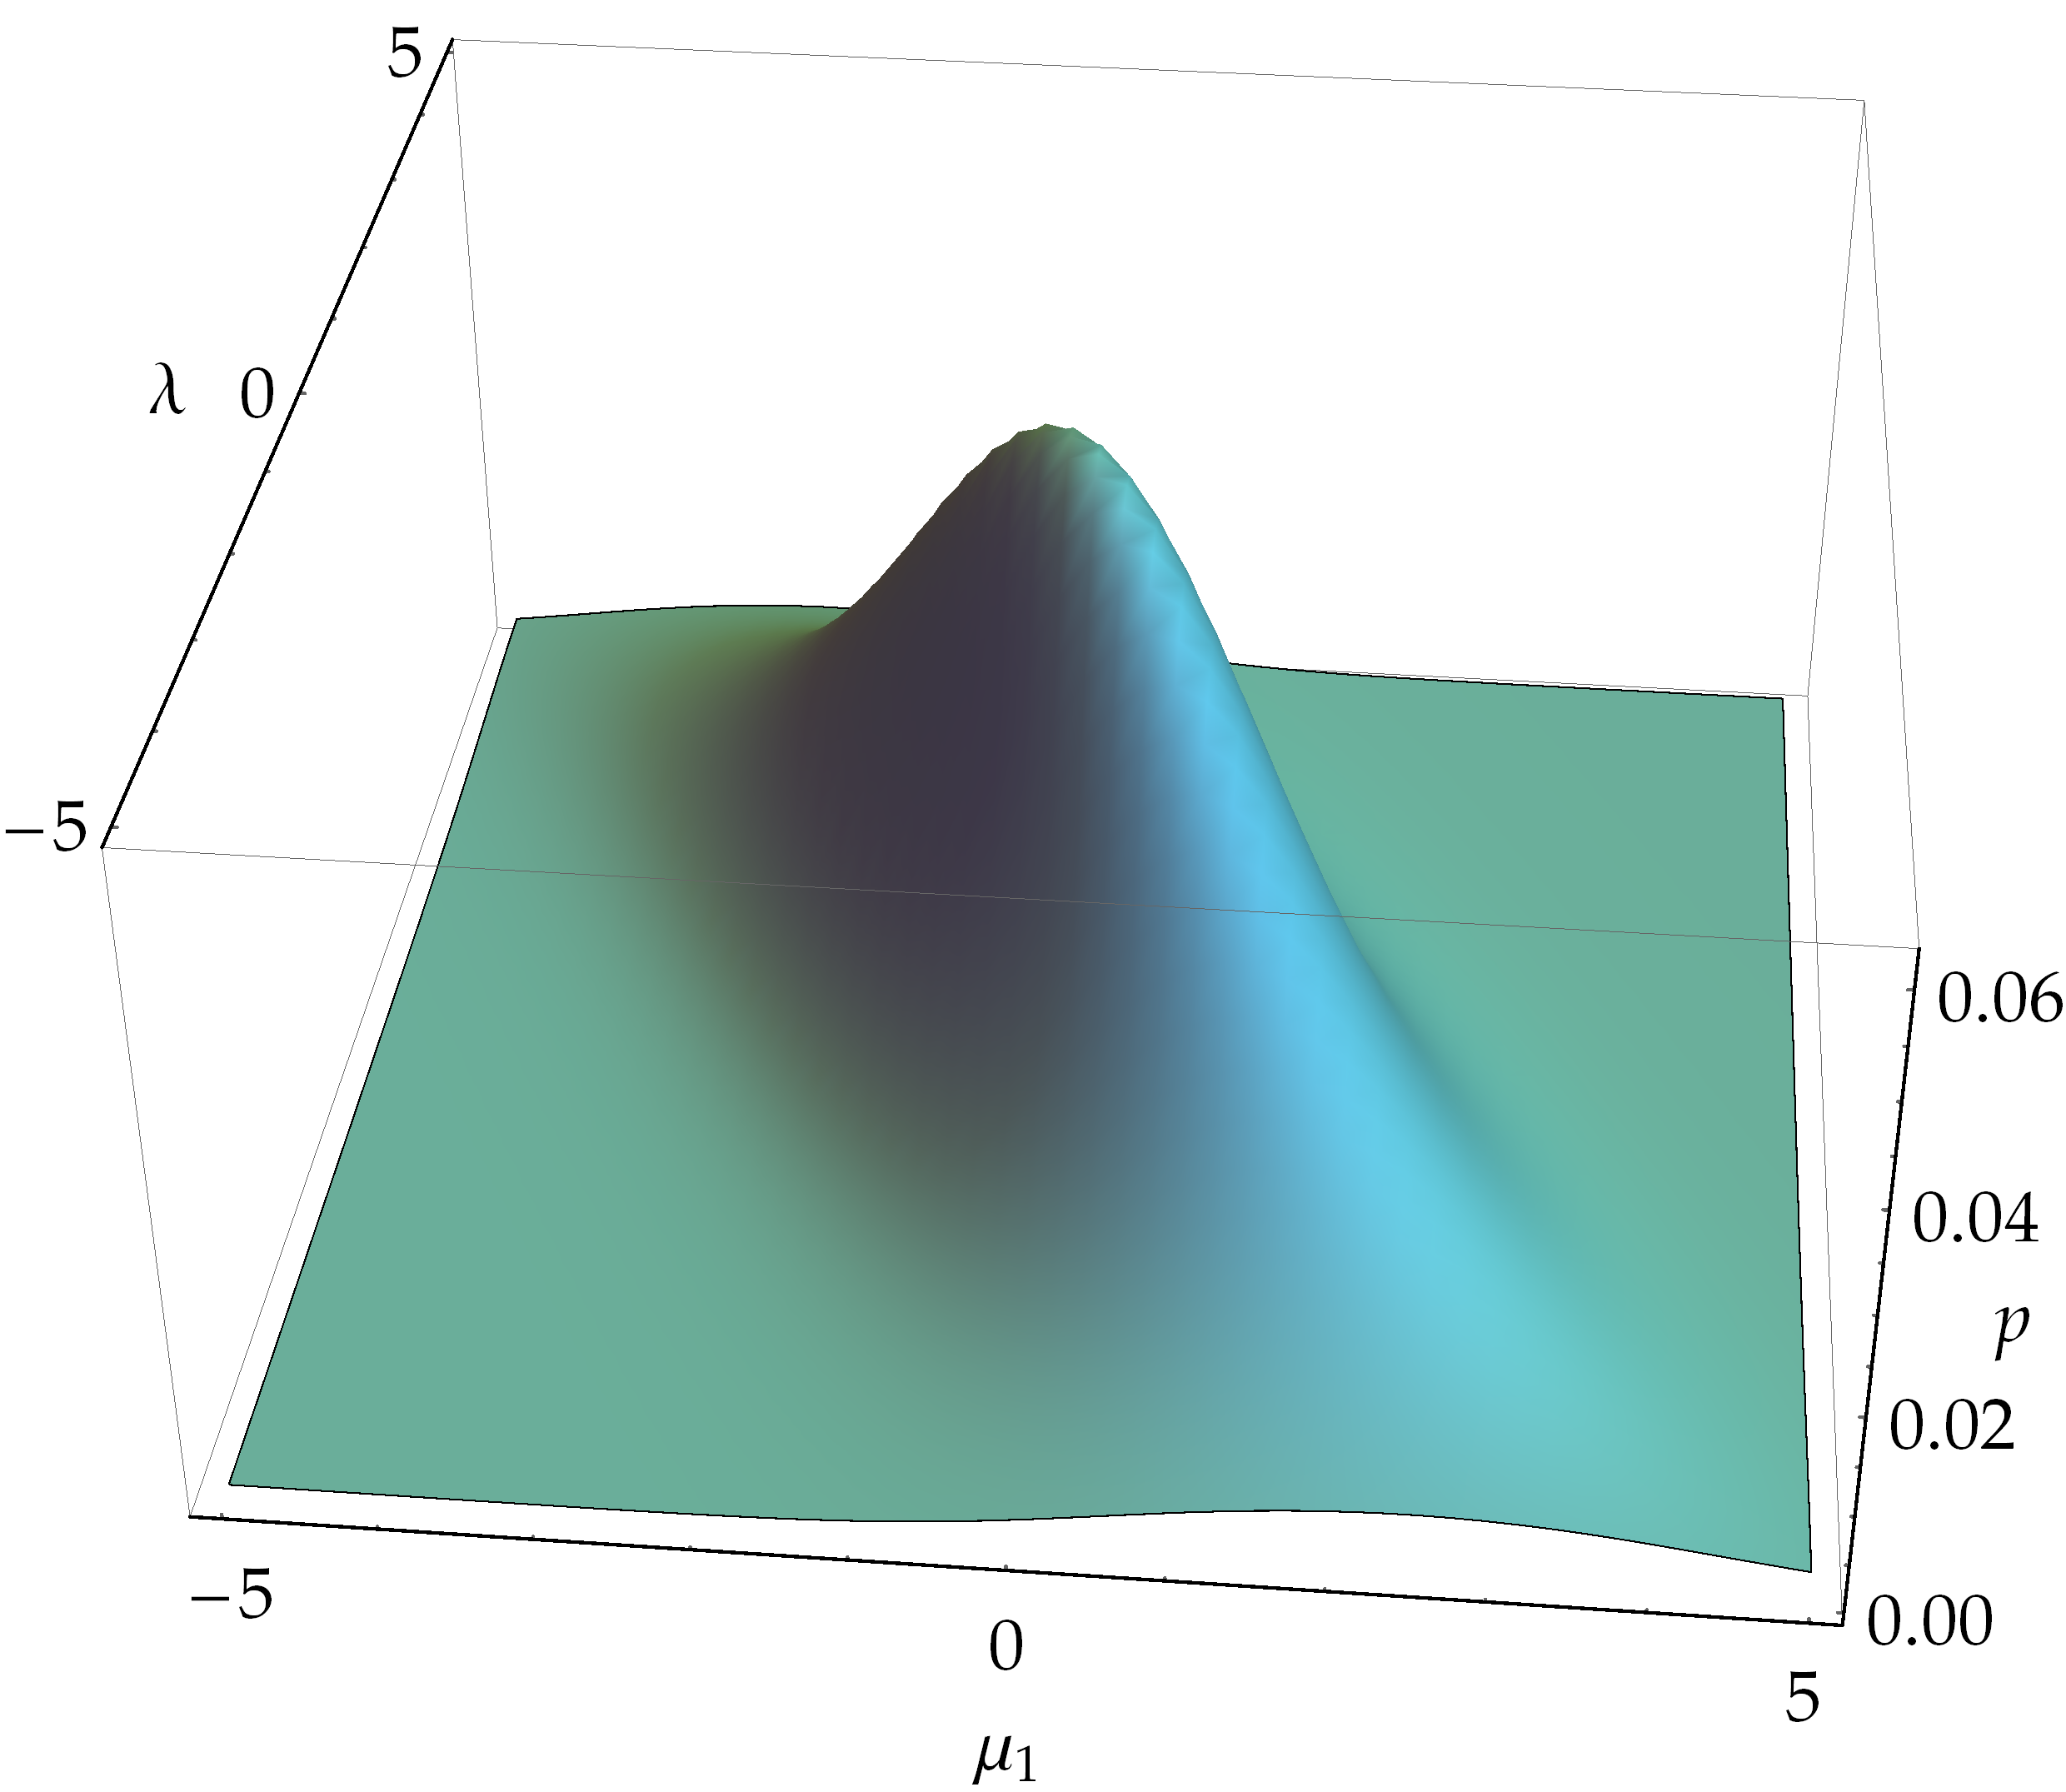
\includegraphics[width=0.75\linewidth]{marginal_flatstat.png}\\
  \caption{}
  \label{fig:marginal_flatstat}
\end{figure}% dimer_study.nb

Comparing the prior parameter density above with the general
formula~\eqref{eq:posterior_density} for the posterior density, we see that
\emph{the prior density $\yIt$  is equivalent to the posterior density
  $\yIth$ conditional on having observed all four possible outcomes once}:
\begin{equation}
  \label{eq:equivalence_prior_postdata}
  \pf(\yth \|\yIt)\,\di\yth =
\pf(\yth \| 00,10,01,11,\yIth)\,\di\yth.
\end{equation}
We can write this as $\yIt = \yIth \land \yA$, where $\yA$ represents the
observation of the four outcomes.

This result is computationally important. If we want to make inferences
conditional on some data $\yD$ using a density constant in $\yt$, we can
use the same algorithms and approximations used for the density constant in
$\yth$, but augmenting the data $\yD$ with the \enquote{auxiliary data} $\yA$.

If it can be proven that the formula for the Jacobian
determinant~\eqref{eq:jacobian_as_probs} holds for any number of units,
then this method requires to add $2^n$ auxiliary data if we consider $n$
units. This should have a big influence on our predictions even when the
observed data are numerous.

\subsection{Explicit formulae for belief update: connection with Dirichlet priors}
\label{sec:explicit_dirichlet}

The three-dimensional family of probabilities $\pf(\ys \| \yth, \yI)$ or
$\pf(\ys \|\yt,\yI)$ covers the full simplex of probability distributions
for the four states of our units. Our model is actually
\enquote{non-parametric}. This is clear from
formulae~\eqref{eq:prob_outcome_from_statistics}: the limit statistics
$\yt$ determine the limit relative frequencies of the four states and vice
versa.

Consider then a new parameterization $\yq\defd(q_1,q_2,\yql)$ defined by
\begin{gather}
  \label{eq:params_q}
  q_1 = m_1-\yl,\quad q_2=m_2-\yl, \quad \yql = \yl,
  \\\shortintertext{and denote}
  q_0 \defd 1-q_1-q_2-\yql.
\end{gather}
In terms of these parameters our three-dimensional family of distributions
is
\begin{multline}
  \label{eq:prob_parametr_q}
  \begin{aligned}
  \pf(\ys \| \yq,\yI) &=
  \begin{cases}
     q_0 &\text{for } \ys=00\\
    q_1 &\text{for } \ys=10\\
    q_2 &\text{for } \ys=01\\
    \yql &\text{for } \ys=11
  \end{cases}
  \\
&\equiv q_{\ys},\quad\text{where $\ys$ is interpreted as a binary number.}  
  \end{aligned}
\end{multline}
The parameters $(q_0,\yq)$ belong to the three-dimensional simplex
\begin{equation}
\simpl \defd \set{\bm{x} \in \RR^4 \suchthat 
  \tsum_{s=1}^4 x_s=1, x_s\ge 0}.
\label{eq:simplex}
\end{equation}

The probability distribution for a sequence of states becomes
\begin{equation}
  \label{eq:predictive_q}
  \pf(\yso{1}, \dotsc, \yso{N} \|\yI )
=\int
\Biggl[  \prod_{i=1}^{N} q_{\ysso{i}} \Biggr]\,
  \pf(\yq \| \yI)\,\di\yq. 
\end{equation}

From \eqn~\eqref{eq:prob_outcome_from_statistics}, the quantities
$(1-q_1-q_2-\yql, q_1, q_2, \yql)$ can be interpreted as the limit relative
frequencies of the states $(00,10,01,11)$, and the parameter density
$\pf(\yq\|\yI)\,\di\yq$ as our uncertainty about these frequencies.

The parameter transformation~\eqref{eq:params_q} has unit Jacobian, so we have
\begin{equation}
  \label{eq:equiv_priors_m_q}
  \pf(\yt \|\yI)\,\di\yt = \pf(\yq \|\yI)\,\di\yq.
\end{equation}
A constant parameter density in $\ym$ is also constant in $\yq$, and is a
special case of the parameter density function
\begin{equation}
  \label{eq:johnson-dirichlet}
  \begin{gathered}
  \pf(\yq \|\yN,\yn, \yI) =
  \frac{\Gamma(\yN)}{\prod_{i=0}^3 \Gamma(\yN\ynn_i)}\,
  \prod_{i=0}^3{q_i}^{\yN\ynn_i-1},\\
\text{with}\quad \yN>0, \yn \defd (\ynn_i) \in \simpl.
\end{gathered}
\end{equation}
This density was used by Laplace \citey{laplace1778_r1781} and motivated by
Johnson \citey{johnson1924,johnson1932c}, and its integrals can be
analytically calculated with Dirichlet's \citey{dirichlet1839}
formula~\eqref{eq:Dirichlet_formula}. This density is commonly called
\enquote{Dirichlet prior}
\cites(see)()[\chap~4]{good1965}{zabell1982,jaynes1986d_r1996,guptaetal2001}
but we'll call it \enquote{Johnson density} here, since he determined its
mathematical form from informational desiderata.

The Johnson density is a conjugate prior
\cites[\chap~9]{degroot1970_r2004}{diaconisetal1979b}: it updates to a
density of the same mathematical form. It leads to probabilities with
closed-form formulae summarized in
appendix~\ref{sec:formulae_johnson_density}. In particular, the posterior
probability distribution for a state is
\newlength{\myl}\settowidth{\myl}{\footnotesize in the $N$ observations}
\begin{equation}
  \label{eq:predictive_q_general}
\begin{gathered}
  \p(\yso{N+1} \| \yso{1}, \dotsc, \yso{N}, \yN, \yn,\yI) =
  \frac{\yN\ynn_{\yso{N+1}} + N\,\yff_{\yso{N+1}}}{\yN+N},
  \\\text{with }
  \yff_{\yso{N+1}} \defd \text{\footnotesize rel. frequency of state $\yso{N+1}$ in
  the $N$ observations}.
  % \Bigl\{
  %   \parbox[c]{\the\myl}{\footnotesize rel. frequency of $\ys$\\ in
  % the $N$ observations}  
\end{gathered}
\end{equation}

\bigskip

The density $\pf(\yt \| \yIt)\,\di\yt = 6\,\di\yt$ is a special case of the
Johnson density with $\yN=4$, $\ynn_i=1/4$. The improper density
$\pf(\yth \| \yIth)\,\di\yth \propto \di\yth$, which by
formula~\eqref{eq:jacobian_as_probs} is like $\pf(\yt \| \yIt)$
\enquote{minus four observations}, corresponds to the improper Johnson
density with $\yN\to 0$, $\ynn_i=1/4$. The formula for the posterior
probabilities~\eqref{eq:predictive_q_general} can be used in both cases.
From that formula with $\yN=4$ it is possible to calculate that the number
of observations after which the posterior probability for a state will be
within 10\% of its relative frequency. For a very high relative frequency
this number is $N\approx 30$; for a very low relative frequency $f$ this
number is $N\approx 10/f$. With $\yN \to 0$ instead the predictive
probability is always equal to the relative frequency -- also meaning that
it is zero for states that haven't yet been observed.


\subsection{Initial information}
\label{sec:initial_info}

If we calculate the 

\begin{figure}%$[t!]%{r}{0.4\linewidth} % with wrapfigure
  \centering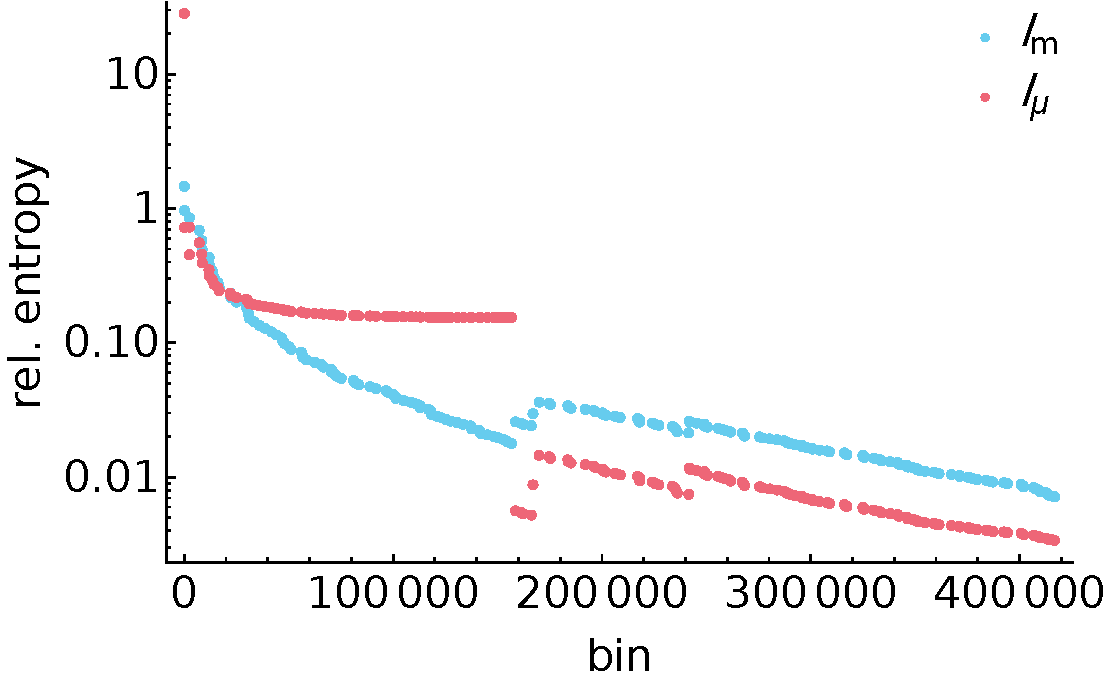
\includegraphics[width=\linewidth]{comp_priors.pdf}\\
  \caption{}
  \label{fig:comp_priors}
\end{figure}% update_2units.nb



\section{[Luca:] Does it make sense to test against computer-generated
  distributions?}
\label{sec:makes_no_sense}

\begin{quotation}\small
  But we must note with sadness that, in much of the current Bayesian
  literature, very little of the orthodox baggage has been cast off. For
  example, it is rather typical to see a Bayesian article start with such
  phrases as: `Let $X$ be a random variable with density function
  $p(x|\theta)$, where the value of the parameter $\theta$ is unknown.
  Suppose this parametric family contains the true distribution of
  $X$\ldots.' Or, one describes a uniform prior $p(\theta|I)$ by saying:
  `$\theta$ is supposed uniformly distributed'. The analytical solutions
  thus obtained will doubtless be a valid Bayesian result; but one is still
  clinging to the orthodox fiction of `random variables' and `true
  distributions'. $\theta$ is simply an unknown constant; it is not
  `distributed' at all. What is `distributed' is our state of knowledge
  about $\theta$: again there is that persistent mind projection fallacy
  that contaminates all of probability theory, leading inexperienced
  readers far astray as to what we are doing. Equally bad, those who commit
  this fallacy seem unaware that this is restricting the application to a
  small fraction of the real situations where the solution might be useful.
  In the vast majority of real applications there are no `random variables'
  (What defines `randomness'?) and no `true distribution' (What defines it?
  What test could we apply to decide whether some proposed distribution is
  or is not the `true' one?); yet probability theory as logic applies to
  all of them.\\\small\mbox{}\hfill Jaynes
  \citey[\sect~17.12]{jaynes1994_r2003}
\end{quotation}

The outcomes of the measurements we make on the system, modelled as a
population of binary units, are produced by utterly complex mechanisms.
They aren't produced by a computer's pseudo-random-number generator. So it
doesn't make sense to check which prior parameter density converges faster
to the parameters of some computer algorithm, because algorithm,
parameters, distribution do not even exist in the real situation.

There's a circularity in using computer-generated outcomes to test which
statistical model or prior density is \enquote{best}. This test would make
sense if the computer algorithm mimicked the outcomes of the real
experiment well. But if we had such an algorithm we wouldn't need any
statistical model to start with.

The use of computer algorithms has a different purpose. A statistical model
or a prior density can be difficult to grasp intuitively. It may have
properties that don't reflect the information or assumptions we had in
mind; in which case it doesn't correctly represent our beliefs. Testing
it against controlled computer-generated outcomes may bring forth such
undesired properties. This is the \enquote{device of imaginary results}
suggested by Good \parentext{\cite*[\sect~4.3]{good1950}; \cite*{good1967b};
  \cite[index in][p.~280]{good1983}; \cite[\chap~5]{jaynes1994_r2003}}.





% The purpose of our probability calculations is not to find some
% \enquote{unknown, true} parameter. Two are two possible purposes:
% \begin{itemize}
% \item to make our best forecast about other outcomes, given the information
%   we have;
% \item to asses the truth of different possible hypotheses, given the outcomes we
%   observe.
% \end{itemize}
% The first corresponds, in formal logic, to deriving a theorem from a set
% of axioms. The second to choosing among axioms by looking at the theorems
% they lead to.



\mynote{To be continued}




%\setlength{\intextsep}{0.5ex}% with wrapfigure
%\begin{figure}[p!]%{r}{0.4\linewidth} % with wrapfigure
%  \centering\includegraphics[trim={12ex 0 18ex 0},clip,width=\linewidth]{maxent_saddle.png}\\
%\caption{***}\label{fig:comparison_a5}
%\end{figure}% exp_family_maxent.nb


\iffalse
\begin{acknowledgements}
  PGLPM thanks Mari \amp\ Miri for continuous encouragement and affection;
  Buster Keaton and Saitama for filling life with awe and inspiration; the
  developers and maintainers of \LaTeX, Emacs, AUC\TeX, Open Science
  Framework, Python, Inkscape, Sci-Hub for making a free and unfiltered
  scientific exchange possible.
%\rotatebox{15}{P}\rotatebox{5}{I}\rotatebox{-10}{P}\rotatebox{10}{\reflectbox{P}}\rotatebox{-5}{O}.
%\sourceatright{\autanet}
\end{acknowledgements}
\fi

% \appendixpage
\renewcommand*{\appendixpagename}{Appendix}
\renewcommand*{\appendixname}{Appendix}
\appendix

\section{Formulae for the Johnson density}
\label{sec:formulae_johnson_density}

Dirichlet's formula
\begin{equation}
  \label{eq:Dirichlet_formula}
  \int_{\simpl} \prod_{i=1}^N {q_{i}}^{x_i-1}\,\di\yq =
  \frac{\prod_i \Gamma(x_i)}{\Gamma\bigl(\sum_i x_i\bigr)}
\end{equation}
allows to calculate all integrals involving the Johnson density.

The posterior density function
\begin{equation}
  \label{eq:posterior_q}
\begin{gathered}
  \pf(\yq \| \yso{1}, \dotsc, \yso{N}, \yN, \yn,\yI)
  = 
  \frac{\Gamma(\yN')}{\prod_i \Gamma(\yN'\ynn_i')}\,
  \prod_{i=0}^{3}{q_i}^{\yN'\ynn_i'-1}
  \\
  \text{with}\quad \yN' =\yN+N,\quad
  \yn'=\frac{\yN\yn+N\yf}{\yN+N},\quad
    \yff_{\ys} \defd\Bigl\{
    \parbox[c]{\the\myl}{\footnotesize rel. frequency of $\ys$\\ in
  the $N$ observations}  
\end{gathered}
\end{equation}
The posterior probability distribution for a state:
\begin{equation}
  \label{eq:predictive_q_general}
  \p(\yso{N+1} \| \yso{1}, \dotsc, \yso{N}, \yN, \yn,\yI) =
  \frac{\yN\ynn_{\yso{N+1}} + N\,\yff_{\yso{N+1}}}{\yN+N}.
\end{equation}



%%%%%%%%%%%%%%% BIB %%%%%%%%%%%%%%%

\defbibnote{prenote}{{\footnotesize (\enquote{de $X$} is listed under D,
    \enquote{van $X$} under V, and so on, regardless of national
    conventions.)\par}}
% \defbibnote{postnote}{\par\medskip\noindent{\footnotesize% Note:
%     \arxivp \mparcp \philscip \biorxivp}}

\printbibliography[prenote=prenote%,postnote=postnote
]


\end{document}
---------- cut text ----------------


Denote by $K(\yav,\ycv;N)$ the number of possible sequences of $N$
observations $(\yso{1}, \dotsc, \yso{N})$ that have statistics
$(\yav,\ycv)$. Note that $\sum_{\yav,\ycv} K(\yav,\ycv; N) = 4^N$, the
total number of possible sequences of $N$ observations. For example, if
$N=4$, there are 12 possible sequences that have statistics $\yavv_1=2/4$,
$\yavv_2=1/4$, $\ycv=1/4$: the sequence $(00,00,10,11)$ and its $4!/2$
distinct permutations; therefore $K(2/4,1/4,1/4; 4)=12$.



, noting that it can be written
\begin{equation}
    \label{eq:component_combination_statistics}
  \pf(\yso{1}, \dotsc, \yso{N} \|\yth, \yI )
  =
%  g\bigl(\yso{i}\bigr)\,
  \frac{  \exp[N\,(
    \mu_1 \yavv_1 + \mu_2 \yavv_2 + \la \ycv)]}{Z(\yth)^N}.
\end{equation}
This probability has the same value for all sequences $(\yso{1}, \dotsc,
\yso{N})$ having the same statistics $(\yav,\ycv)$. Therefore, the
probability of observing a particular statistics, given $\yth$, is
\begin{equation}
  \label{eq:prob_statistics_param}
  \pf(\yav,\ycv \| \yth,\yI) =
  K(\yav,\ycv; N) \,
  \frac{  \exp[N\,(
    \mu_1 \yavv_1 + \mu_2 \yavv_2 + \la \ycv)]}{Z(\yth)^N},
\end{equation}
and considering the convex combination we have
\begin{equation}
  \label{eq:prob_statistics}
  \pf(\yav,\ycv \| \yI) =
  K(\yav,\ycv; N) 
\int  \frac{  \exp[N\,(
  \mu_1 \yavv_1 + \mu_2 \yavv_2 + \la \ycv)]}{Z(\yth)^N}
\, \pf(\yth \|\yI) \, \di\yth.
\end{equation}

When $N$ is large, the exponential term with the largest argument dominates
as $\yth$ varies. The parameter values $\ythm$ of this term are therefore
\begin{equation}
  \label{eq:max_posterior}
  \ythm \defd \argsup_{\yth}
 [ \mu_1 \yavv_1 + \mu_2 \yavv_2 + \la \ycv -\ln Z(\yth)],
\end{equation}
and they can be shown to be unique \citep{meadetal1984}; in fact they are
implicitly given by the equations \citep{meadetal1984,portamana2017b}
\begin{gather}
  \label{eq:change_coords}
  \begin{gathered}
    m_1 = \frac{\de\ln Z(\yth)}{\de \mu_1}
    \equiv \expe{s_1 \|\yth,\yI},
    \qquad
  m_2 = \frac{\de\ln Z(\yth)}{\de \mu_2}
    \equiv \expe{s_2 \|\yth,\yI},\\
  \yl = \frac{\de\ln Z(\yth)}{\de\la}
    \equiv \expe{s_1 s_2\|\yth,\yI}.
  \end{gathered}
  \\[2\jot]
  \label{eq:max_params}
  \text{for}\qquad
  (m_1,m_2,\yl) = (\yavv_1,\yavv_2,\ycv),
  \quad \yth=\ythm.
\end{gather}
The system of equations~\eqref{eq:change_coords} gives a one-one
correspondence between the parameters $\yt\defd(m_1, m_2,\yl)$ and
$\yth \defd(\mu_1, \mu_2, \la)$. The latter belong to $\RR^3$; the former
to the bounded domain
\begin{equation}
  \label{eq:domain_newcoords}
  0\le m_1,m_2 \le 1,
  \qquad
  \max(0,1-m_1-m_2) \le \yl \le \min(m_1,m_2).
\end{equation}



\subsection{Other prior parameter densities}
\label{sec:other_priors}


As noted before, the parameters $\yth$ are just coordinates in a manifold
of distributions for $\ys$. A constant density in these coordinates
corresponds to an non-constant density in other coordinates. But are these
coordinates \enquote{special} in any way, to consider a constant density in
them? Are there other coordinates in which it makes more sense to consider
a constant density? How does a different choice affect our inference about
$\ys$?

To consider other coordinates it is useful to give the predictive
formula~\eqref{eq:predictive_KP} a particular interpretation.

First of all it must be noted that each choice of parameters $\yth$ gives
a distribution
\begin{equation}
  \label{eq:distr_simple_s}
  \pf(\ys \|\yth, \yI)
  =
  \frac{  \exp\bigl(
      \mu_1 \ysso{i}_1 + \mu_2 \ysso{i}_2 + \la \ysso{i}_1 \ysso{i}_2
      \bigr) }{Z(\yth)}
\end{equation}
with different first and second moments
\begin{equation}
  \label{eq:moments}
  \begin{aligned}
    \expe{\ys \|\yth, \yI} &\defd
    \sum_{\ys} \ys\, \pf(\ys \|\yth, \yI),
\\
    \expe{s_1 s_2 \|\yth, \yI} &\defd
    \sum_{\ys} s_1 s_2\, \pf(\ys \|\yth, \yI).
  \end{aligned}
\end{equation}
In other words the set $\yth \in \RR^3$ is in one-one correspondence with
the possible values of the three expectations above. We can therefore
introduce coordinates $\yt \defd (m_1, m_2, \yl)$ that identify the
distributions above via the equations
\begin{equation}
  \label{eq:tranf_coord}
  \begin{split}
  m_1 &= \expe{s_1 \|\yth, \yI} \equiv
  \frac{\exp(\mu_1) + \exp(\mu_1 + \mu_2 + \la)}{Z(\mu_1,\mu_2,\la)},\\
  m_2 &= \expe{s_2 \|\yth, \yI} \equiv
  \frac{\exp(\mu_2) + \exp(\mu_1 + \mu_2 + \la)}{Z(\mu_1,\mu_2,\la)},\\
  \qquad
  \yl &= \expe{s_1 s_2 \|\yth, \yI} \equiv
  \frac{\exp(\mu_1 + \mu_2 + \la)}{Z(\mu_1,\mu_2,\la)},
\end{split}
\end{equation}
which are coordinate transformations with the inverse
\begin{equation}
  \label{eq:inverse_tranf_coord}
  \begin{gathered}
    \mu_1 =\ln\frac{m_1-\yl}{1+\yl-m_1-m_2},\qquad
    \mu_2 =\ln\frac{m_2-\yl}{1+\yl-m_1-m_2},\\[\jot]
\la =\ln\frac{(1+\yl-m_1-m_2)\,\yl}{(m_1-\yl)\,(m_2-\yl)}.
\end{gathered}
\end{equation}

In terms of the coordinates $\yt$ the family of probability distributions
for $\ys$ has the form
\begin{multline}
  \label{eq:prob_family_m}
  \pf(\ys \| \yt,\yI) =
  (1+\yl-m_1-m_2)\times{}\\
  \biggl(\frac{m_1-\yl}{1+\yl-m_1-m_2} \biggr)^{s_1}\,
  \biggl( \frac{m_2-\yl}{1+\yl-m_1-m_2}  \biggr)^{s_2}\,
  \Biggl[ \frac{(1+\yl-m_1-m_2)\,\yl}{(m_1-\yl)\,(m_2-\yl)} \Biggr]^{s_1 s_2}
  \\[\jot]
  {}\equiv
  \yl^{s_1 s_2}\,
  (m_1-\yl)^{s_1-s_1 s_2}\,
  (m_2-\yl)^{s_2-s_1 s_2}\,
  (1+\yl-m_1-m_2)^{1-s_1-s_2+s_1 s_2}.
\end{multline}


%%% Local Variables: 
%%% mode: LaTeX
%%% TeX-PDF-mode: t
%%% TeX-master: t
%%% End: 
